\documentclass[a4paper,12pt]{article}

\usepackage{newtxtext}
\usepackage[margin=1in]{geometry}
\usepackage{graphicx}
\usepackage{amsmath}
\usepackage{amssymb}
\usepackage{booktabs}
\usepackage{longtable}
\usepackage{array}
\usepackage{tabularx}
\usepackage{float}
\usepackage{caption}
\usepackage{subcaption}
\usepackage{hyperref}
\usepackage{xurl}
\usepackage{setspace}
\usepackage{makecell}
\usepackage{enumitem}
\usepackage{tikz}
\usetikzlibrary{arrows.meta,calc,positioning}

\hypersetup{
    colorlinks=true,
    linkcolor=black,
    citecolor=black,
    urlcolor=blue
}

\setlength{\parindent}{2em}
\setlength{\parskip}{0.3em}
\setstretch{1.25}
\setlength{\emergencystretch}{2em}
\renewcommand{\arraystretch}{1.15}
\renewcommand{\UrlFont}{\ttfamily\small}
\Urlmuskip=0mu plus 1mu\relax
\graphicspath{{Figures/}}
\newcommand{\code}[1]{\nolinkurl{#1}}
\newcolumntype{L}[1]{>{\raggedright\arraybackslash}p{#1}}
\newcolumntype{Y}{>{\raggedright\arraybackslash}X}

\tikzset{
    seq participant/.style={
        draw,
        rounded corners=2pt,
        fill=black!5,
        minimum width=1.75cm,
        minimum height=0.72cm,
        align=center,
        font=\scriptsize
    },
    seq lifeline/.style={gray!60, dashed},
    seq call/.style={-{Latex[length=2mm,width=1.2mm]}, semithick},
    seq reply/.style={-{Latex[length=2mm,width=1.2mm]}, semithick, dashed},
    seq note/.style={
        draw,
        rounded corners=2pt,
        fill=yellow!12,
        text width=3.9cm,
        align=left,
        inner sep=3pt,
        font=\scriptsize
    },
    seq note wide/.style={
        draw,
        rounded corners=2pt,
        fill=yellow!12,
        text width=6.8cm,
        align=left,
        inner sep=3pt,
        font=\scriptsize
    },
    arch box/.style={
        draw,
        rounded corners=2pt,
        fill=blue!7,
        minimum width=3.5cm,
        minimum height=1.0cm,
        text width=3.2cm,
        align=center,
        font=\small
    },
    arch io/.style={
        draw,
        rounded corners=2pt,
        fill=green!10,
        minimum width=3.8cm,
        minimum height=1.0cm,
        text width=3.5cm,
        align=center,
        font=\small
    },
    arch accent/.style={
        draw,
        rounded corners=2pt,
        fill=orange!12,
        minimum width=3.5cm,
        minimum height=1.0cm,
        text width=3.2cm,
        align=center,
        font=\small
    },
    arch arrow/.style={-{Latex[length=2.2mm,width=1.4mm]}, semithick},
    arch feedback/.style={-{Latex[length=2.2mm,width=1.4mm]}, semithick, dashed, color=orange!70!black}
}

\newcommand{\overallArchitectureFigure}{
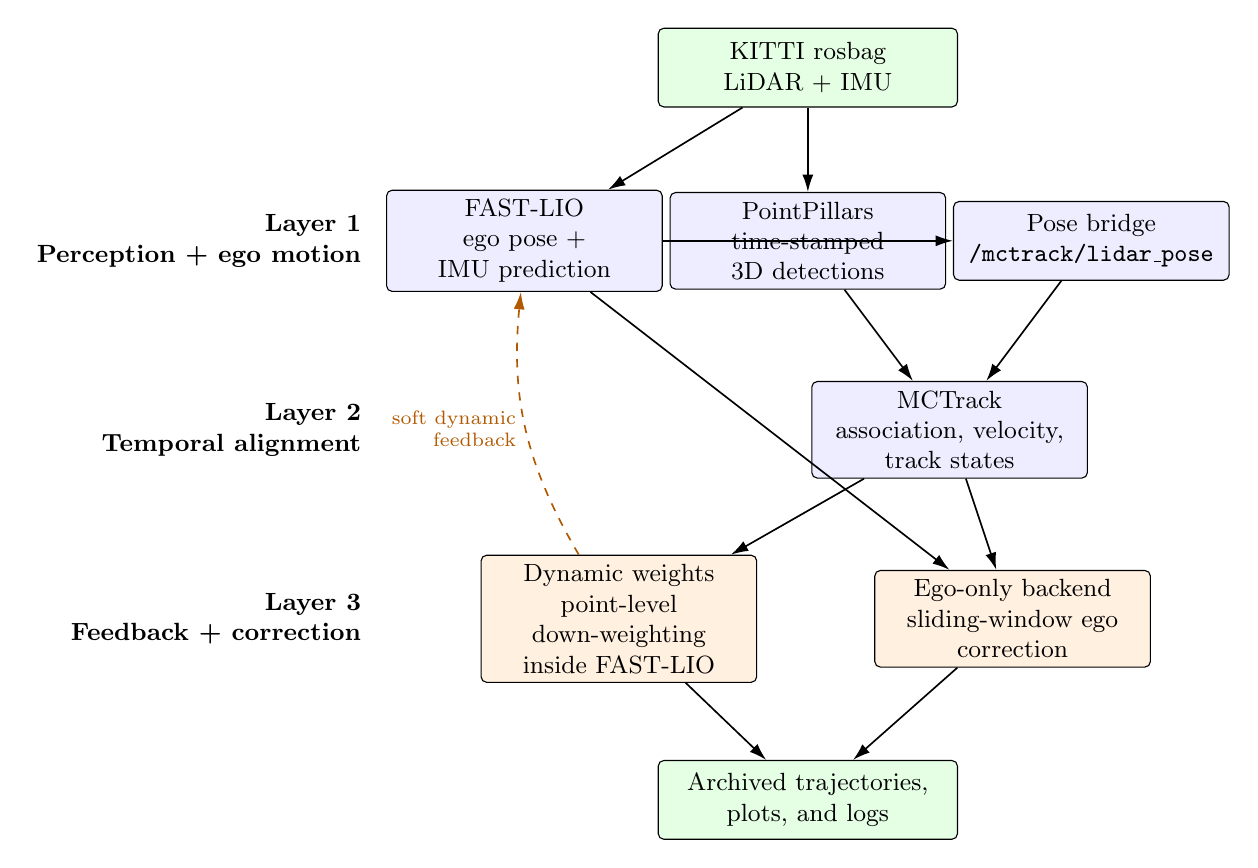
\begin{tikzpicture}[x=1cm,y=1cm]
    \node[arch io] (input) at (0,0) {KITTI rosbag\\LiDAR + IMU};
    \node[arch box] (fl) at (-3.6,-2.2) {FAST-LIO\\ego pose + IMU prediction};
    \node[arch box] (pp) at (0,-2.2) {PointPillars\\time-stamped 3D detections};
    \node[arch box] (bridge) at (3.6,-2.2) {Pose bridge\\\texttt{/mctrack/lidar\_pose}};
    \node[arch box] (mc) at (1.8,-4.6) {MCTrack\\association, velocity,\\track states};
    \node[arch accent] (weight) at (-2.4,-7.0) {Dynamic weights\\point-level down-weighting\\inside FAST-LIO};
    \node[arch accent] (backend) at (2.6,-7.0) {Ego-only backend\\sliding-window ego\\correction};
    \node[arch io] (out) at (0,-9.3) {Archived trajectories,\\plots, and logs};

    \node[font=\small\bfseries, anchor=east, align=right] at (-5.55,-2.2) {Layer 1\\Perception + ego motion};
    \node[font=\small\bfseries, anchor=east, align=right] at (-5.55,-4.6) {Layer 2\\Temporal alignment};
    \node[font=\small\bfseries, anchor=east, align=right] at (-5.55,-7.0) {Layer 3\\Feedback + correction};

    \draw[arch arrow] (input) -- (fl);
    \draw[arch arrow] (input) -- (pp);
    \draw[arch arrow] (fl) -- (bridge);
    \draw[arch arrow] (bridge) -- (mc);
    \draw[arch arrow] (pp) -- (mc);
    \draw[arch arrow] (mc) -- (weight);
    \draw[arch arrow] (mc) -- (backend);
    \draw[arch arrow] (fl) -- (backend);
    \draw[arch arrow] (weight) -- (out);
    \draw[arch arrow] (backend) -- (out);
    \draw[arch feedback] (weight) to[bend left=18] node[midway,left,font=\scriptsize,align=right] {soft dynamic\\feedback} (fl);
\end{tikzpicture}
}

\newcommand{\onlineSequenceFigure}{
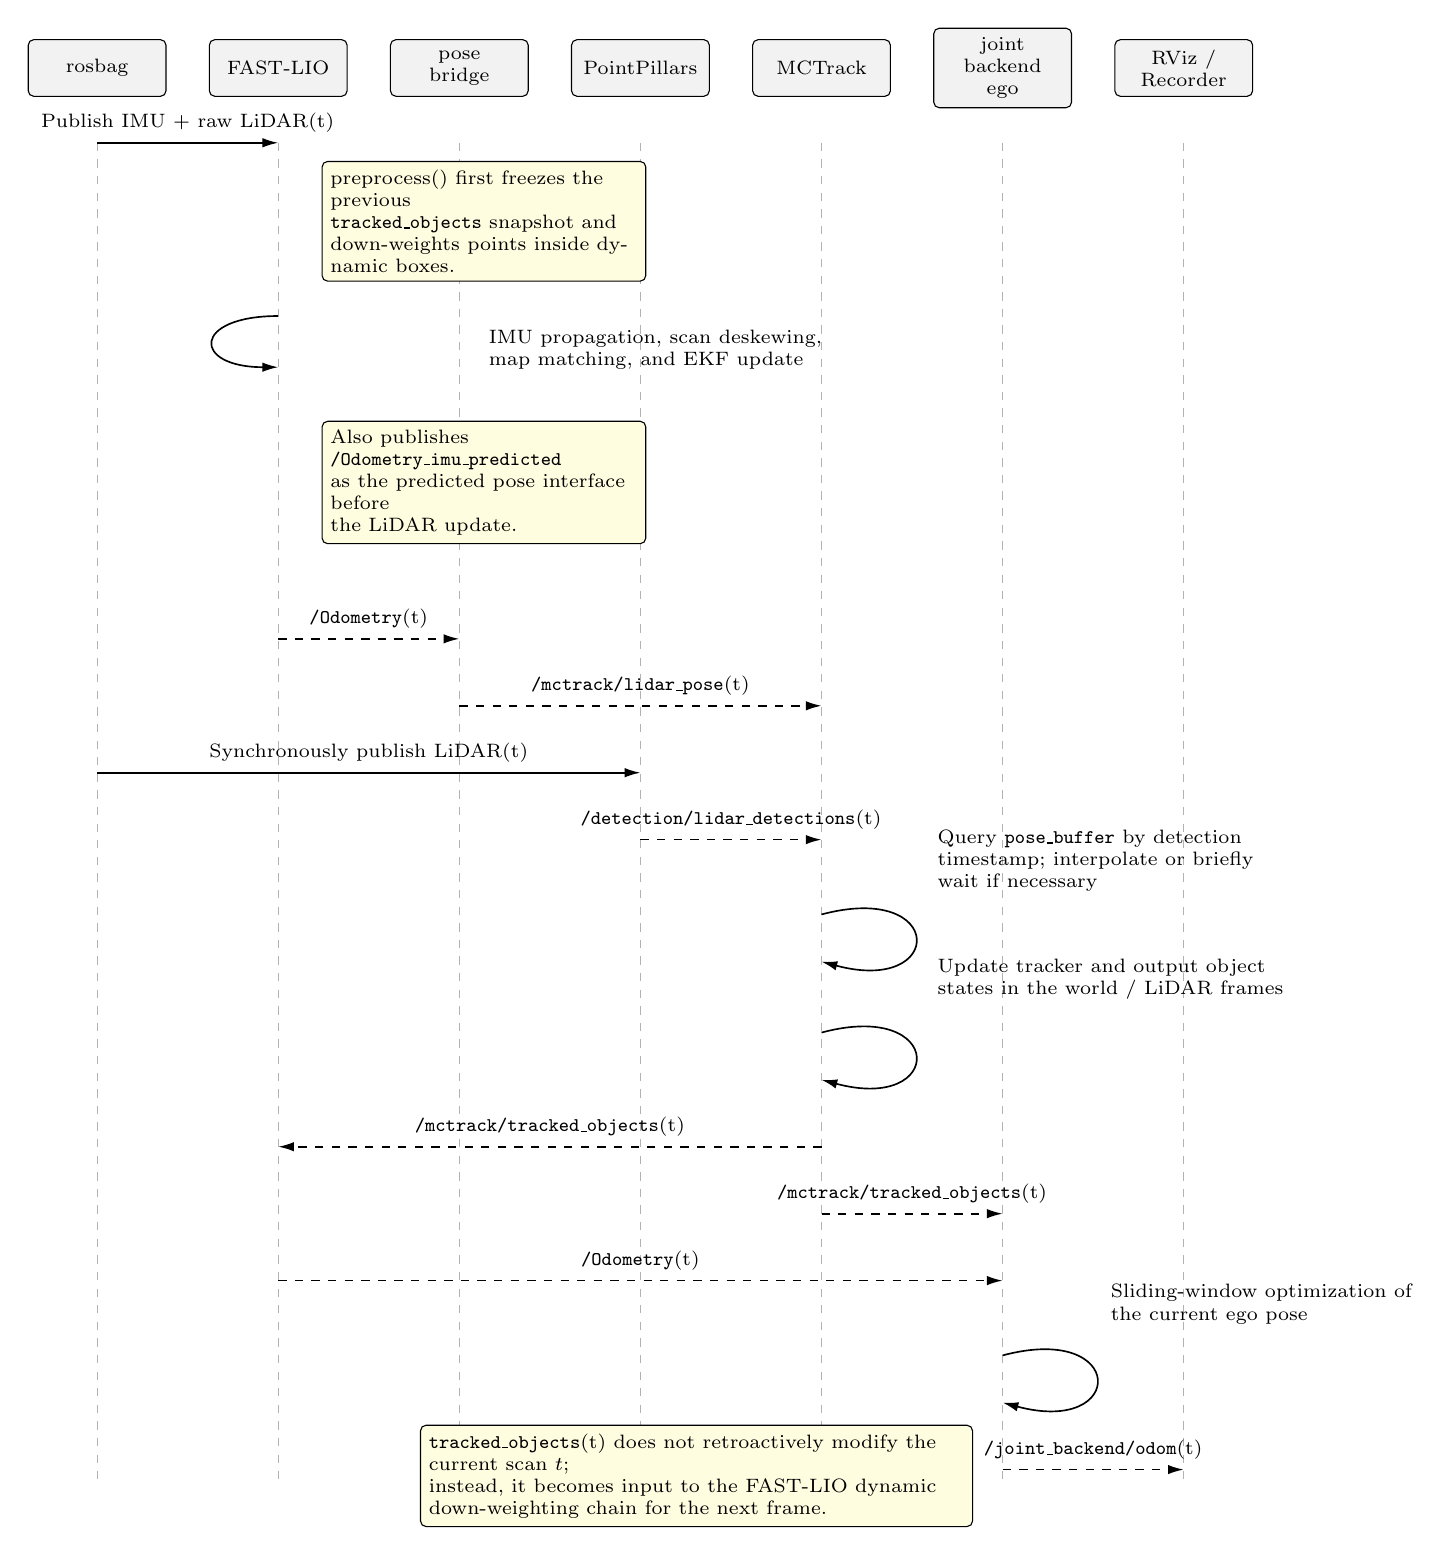
\begin{tikzpicture}[x=1cm,y=1cm]
    \node[seq participant] (bag) at (0.0,0) {rosbag};
    \node[seq participant] (fl) at (2.3,0) {FAST-LIO};
    \node[seq participant] (br) at (4.6,0) {pose\\bridge};
    \node[seq participant] (pp) at (6.9,0) {PointPillars};
    \node[seq participant] (mc) at (9.2,0) {MCTrack};
    \node[seq participant] (jb) at (11.5,0) {joint\\backend\\ego};
    \node[seq participant] (out) at (13.8,0) {RViz /\\Recorder};

    \coordinate (seqtop) at (0,-0.95);
    \foreach \p/\name in {bag/bagline,fl/flline,br/brline,pp/ppline,mc/mcline,jb/jbline,out/outline} {
        \path (\p.center |- seqtop) coordinate (\name);
        \draw[seq lifeline] (\name) -- ++(0,-17.0);
    }

    \draw[seq call]
        (bagline) --
        node[above,font=\scriptsize] {Publish IMU + raw LiDAR(t)}
        (flline);

    \node[seq note, anchor=north west] at (2.85,-1.18) {preprocess() first freezes the previous\\\texttt{tracked\_objects} snapshot and\\down-weights points inside dynamic boxes.};

    \draw[seq call]
        ($(flline)+(0,-2.2)$)
        .. controls ($(flline)+(-1.1,-2.2)$) and ($(flline)+(-1.1,-2.85)$)
        .. ($(flline)+(0,-2.85)$);
    \node[font=\scriptsize,align=left,anchor=west] at (4.85,-3.58) {IMU propagation, scan deskewing,\\map matching, and EKF update};

    \node[seq note, anchor=north west] at (2.85,-4.48) {Also publishes \texttt{/Odometry\_imu\_predicted}\\as the predicted pose interface before\\the LiDAR update.};

    \draw[seq reply]
        ($(flline)+(0,-6.3)$) --
        node[above,font=\scriptsize] {\texttt{/Odometry}(t)}
        ($(brline)+(0,-6.3)$);

    \draw[seq reply]
        ($(brline)+(0,-7.15)$) --
        node[above,font=\scriptsize] {\texttt{/mctrack/lidar\_pose}(t)}
        ($(mcline)+(0,-7.15)$);

    \draw[seq call]
        ($(bagline)+(0,-8.0)$) --
        node[above,font=\scriptsize] {Synchronously publish LiDAR(t)}
        ($(ppline)+(0,-8.0)$);

    \draw[seq reply]
        ($(ppline)+(0,-8.85)$) --
        node[above,font=\scriptsize] {\texttt{/detection/lidar\_detections}(t)}
        ($(mcline)+(0,-8.85)$);

    \draw[seq call]
        ($(mcline)+(0,-9.8)$) to[out=15,in=345,looseness=7]
        ($(mcline)+(0,-10.4)$);
    \node[font=\scriptsize,align=left,anchor=west] at (10.55,-10.07) {Query \texttt{pose\_buffer} by detection\\timestamp; interpolate or briefly\\wait if necessary};

    \draw[seq call]
        ($(mcline)+(0,-11.3)$) to[out=15,in=345,looseness=7]
        ($(mcline)+(0,-11.9)$);
    \node[font=\scriptsize,align=left,anchor=west] at (10.55,-11.57) {Update tracker and output object\\states in the world / LiDAR frames};

    \draw[seq reply]
        ($(mcline)+(0,-12.75)$) --
        node[above,font=\scriptsize] {\texttt{/mctrack/tracked\_objects}(t)}
        ($(flline)+(0,-12.75)$);

    \draw[seq reply]
        ($(mcline)+(0,-13.6)$) --
        node[above,font=\scriptsize] {\texttt{/mctrack/tracked\_objects}(t)}
        ($(jbline)+(0,-13.6)$);

    \draw[seq reply]
        ($(flline)+(0,-14.45)$) --
        node[above,font=\scriptsize] {\texttt{/Odometry}(t)}
        ($(jbline)+(0,-14.45)$);

    \draw[seq call]
        ($(jbline)+(0,-15.4)$) to[out=15,in=345,looseness=7]
        ($(jbline)+(0,-16.0)$);
    \node[font=\scriptsize,align=left,anchor=west] at (12.75,-15.7) {Sliding-window optimization of\\the current ego pose};

    \draw[seq reply]
        ($(jbline)+(0,-16.85)$) --
        node[above,font=\scriptsize] {\texttt{/joint\_backend/odom}(t)}
        ($(outline)+(0,-16.85)$);

    \node[seq note wide, anchor=north west] at (4.1,-17.23) {\texttt{tracked\_objects}(t) does not retroactively modify the current scan $t$;\\instead, it becomes input to the FAST-LIO dynamic down-weighting chain for the next frame.};
\end{tikzpicture}
}

\newcommand{\onlineResultFigure}[1]{
\begin{figure}[!h]
    \centering
    \begin{subfigure}[t]{0.49\textwidth}
        \centering
        
\includegraphics[width=\linewidth]{../Results/#1_results/Online/evaluation_result.png}
        \caption{Online front-end comparison}
    \end{subfigure}
    \hfill
    \begin{subfigure}[t]{0.49\textwidth}
        \centering
        
\includegraphics[width=\linewidth]{../Results/#1_results/Online/evaluation_joint_backend.png}
        \caption{Joint backend evaluation}
    \end{subfigure}

    \vspace{0.8em}

    \begin{subfigure}[t]{0.58\textwidth}
        \centering
        
\includegraphics[width=\linewidth]{../Results/#1_results/Online/ablation_bar.png}
        \caption{ATE/RPE bar comparison}
    \end{subfigure}
    \caption{Complete online experimental results for Sequence #1.}
\end{figure}
}

\title{LiDAR SLAM with Multiple Object Tracking(MOT) for Autonomous Driving}
\author{ME5400 Project\\Wu Zining (A0294373W)}
\date{\today}

\makeatletter
\newcommand{\makecoverpage}{
\begin{titlepage}
    \centering
    \vspace*{2.0cm}
    
\includegraphics[width=0.58\textwidth]{nus_logo_cover.jpg}\par

    \vspace{2.6cm}
    {\bfseries\fontsize{22}{30}\selectfont
    \parbox{0.9\textwidth}{\centering \@title}\par}

    \vfill
    {\Large \@author \par}
    \vspace{0.8cm}
    {\large \@date \par}
\end{titlepage}
}
\makeatother

\begin{document}
\hypersetup{pageanchor=false}
\makecoverpage
\hypersetup{pageanchor=true}
\tableofcontents
\newpage
\setcounter{page}{1}

\begin{abstract}
This report studies how to improve LiDAR SLAM localization accuracy under dynamic-object interference. Dynamic vehicles, pedestrians, and other traffic participants violate the static-world assumption on which SLAM relies, causing map contamination, registration degradation, and trajectory drift. To address this issue, the project uses FAST-LIO as the main localization backbone and organizes PointPillars and MCTrack as an object-level dynamic-information module: PointPillars provides time-stamped 3D detections, and MCTrack turns them into temporally propagated object states. These object cues are first used for soft dynamic down-weighting in the front end to reduce the misleading effect of dynamic points on scan matching. They are also sent to an ego-only exploratory sliding-window backend to test whether object observations can provide additional constraints.

All quantitative discussion is based on archived online results under \texttt{Results/} for seven selected KITTI Tracking sequences: 0003, 0006, 0007, 0009, 0010, 0013, and 0020. These sequences cover different road types, dynamic intensities, and drift conditions, so within the current repository they form a meaningful multi-sequence ``multi-scene'' validation inside KITTI rather than a claim of cross-dataset generalization. The report emphasizes both algorithmic intent and engineering realization, including ROS interfaces, time synchronization, pose buffering, standardized result archiving, and failure-mode analysis. On this seven-sequence online slice, the front-end configuration \texttt{FAST-LIO+MCTrack} improves ATE RMSE over the pure FAST-LIO baseline in every case, showing that the most stable and best-supported gain comes from object-aware front-end dynamic down-weighting. The exploratory joint backend can help on some drift-dominated sequences, but it is less stable and can fail when velocity extrapolation, timestamp alignment, or object gating are unreliable; Sequence 0009 is the clearest example. Accordingly, the report does not frame the project as a complete SLAMMOT system. Instead, it presents a reproducible experimental platform designed around localization-accuracy improvement in dynamic scenes, clarifying when object-level dynamic information helps localization and when it introduces new uncertainty. The full code, scripts, and experiment structure are available at \url{https://github.com/XC-CN/ME5400}.
\end{abstract}

\noindent\textbf{Keywords:} FAST-LIO; dynamic-scene SLAM; localization-accuracy improvement; object-aware dynamic suppression; KITTI multi-sequence validation; ROS reproducibility

\section{Introduction}
In dynamic road scenes, LiDAR SLAM typically assumes that most observed geometry is static. Vehicles, pedestrians, cyclists, and other traffic participants continually violate this assumption, causing dynamic points to be written into the map and leading to registration degradation, accumulated pose drift, and reduced cross-scene stability. For autonomous-driving workloads, this is not a peripheral issue but a core limit on localization accuracy.

Accordingly, the project does not treat building a complete SLAM+MOT system as its primary goal. Instead, detection and tracking are treated as object-level sources of dynamic information that serve localization. The system uses FAST-LIO~\cite{fastlio2} as the main localization backbone, PointPillars~\cite{pointpillars} to produce 3D detections, and MCTrack~\cite{mctrack} to turn discrete detections into coherent track states. These object states then influence localization in two ways: they are converted into soft dynamic weights inside the FAST-LIO front end to conservatively suppress dynamic regions during scan matching, and they are also sent to an ego-only joint backend as an exploratory extension that tests whether object observations can provide additional constraints in drift-dominated scenes. To balance the course schedule and engineering robustness, the project adopts soft down-weighting and a loosely coupled message loop instead of a tightly coupled object-centric graph.

The project therefore pursues four coupled objectives: the \textbf{research objective} tests whether object-level dynamic information can stably improve LiDAR SLAM localization accuracy in dynamic scenes; the \textbf{engineering objective} builds a repeatable ROS pipeline with clear module boundaries; the \textbf{evaluation objective} analyzes how stable that gain is across KITTI multi-sequence scenes, together with its applicability and failure boundaries; and the \textbf{diagnostic objective} exposes the main vulnerabilities of the exploratory joint backend under velocity extrapolation, time alignment, and gating uncertainty.

In more concrete terms, the contributions of the current report and implementation can be summarized as follows.
\begin{itemize}[leftmargin=2em]
    \item A complete ROS-based integration in which FAST-LIO acts as the main localization backbone while PointPillars and MCTrack provide object-level dynamic observations through project-defined messages.
    \item An object-aware front-end loop in which FAST-LIO poses stabilize cross-frame association in MCTrack, and MCTrack outputs are converted into point-level soft weights inside FAST-LIO preprocessing.
    \item A script-driven experiment framework supporting one-click switching between baseline and optimized runs, standardized archiving under \texttt{Results/}, and unified multi-sequence quantitative evaluation.
    \item A failure-aware analysis showing that object-aware front-end dynamic down-weighting is the most stable current source of localization improvement, whereas the exploratory backend remains fragile under velocity extrapolation and timing uncertainty.
\end{itemize}

The choice of KITTI Tracking as the main validation dataset is deliberate because different sequences cover different road types, dynamic intensities, and drift conditions (here: 0003, 0006, 0007, 0009, 0010, 0013, and 0020), which together form a meaningful ``multi-scene'' localization testbed within the current repository~\cite{kitti}. \textbf{This report is not written as a claim of state-of-the-art performance,} nor does it treat multi-object tracking itself as the end goal. Instead, it documents an engineering prototype designed around improving localization accuracy in dynamic scenes and clarifies when object-level dynamic information helps localization and when it adds uncertainty.

\section{Related Work Analysis}
To position the project more carefully, related work is better organized around one question: how dynamic information is used to improve localization, rather than treating SLAM and MOT as two equal end goals. The first group of methods addresses \textbf{dynamic-scene SLAM} directly by removing, segmenting, restoring, or down-weighting moving regions so that pose estimation is less contaminated. The second group moves toward \textbf{object-aware joint estimation}, where object states, association confidence, or motion priors are allowed to enter localization and optimization more directly. The present project lies between these two groups: it no longer treats dynamic objects merely as points to delete, but it is not yet a full object-centric joint optimizer. A useful comparison should therefore focus on whether dynamic information acts directly on localization, what system complexity that requires, and whether the design remains practical in real-time settings.

\begin{table}[H]
    \centering
    \caption{Representative dynamic-scene SLAM and object-aware joint-estimation methods relevant to the localization-accuracy focus of this report}
    \label{tab:slammot_related_work}
    \footnotesize
    \setlength{\tabcolsep}{5pt}
    \begin{tabularx}{\textwidth}{p{1.9cm} p{2.3cm} p{2.3cm} p{1.7cm} p{2.0cm} X}
        \toprule
        Work & Sensors / front-end & Dynamic handling & Acts directly on localization? & Real-time / complexity & Relevance to this report \\
        \midrule
        StaticFusion & RGB-D; dense direct method & Joint segmentation and background fusion & Yes & Real-time dense mapping~\cite{staticfusion} & Shows that conservative background preservation and weighted treatment can directly improve localization. \\
        DS-SLAM & Vision; ORB-SLAM2 + semantic thread & Semantic filtering + motion consistency & Yes & Multi-threaded and engineering-friendly~\cite{ds-slam} & Shows that a loosely coupled system can still improve localization robustness in dynamic scenes. \\
        DynaSLAM & Vision; ORB-SLAM2 family & Dynamic detection + background inpainting & Yes & Slower but accurate~\cite{dynaslam} & Represents a strong baseline that treats dynamic objects mainly as localization disturbances. \\
        Conf SLAMMOT & LiDAR; LiDAR odometry & Confidence-guided association and object factors & Yes & Tightly coupled and high-complexity~\cite{confslammot} & Suggests that object confidence should scale localization constraints rather than only filter objects. \\
        LIMOT & LiDAR+IMU; LIO & Joint real-time LIO and MOT & Yes & Real-time but implementation-heavy~\cite{limot} & Closest tightly coupled long-term reference for this project. \\
        IMM-SLAMMOT & Stereo vision; ORB-SLAM2 & Multiple motion-model switching & Yes & Stronger modeling, higher cost~\cite{imm-slammot} & Shows why a single constant-velocity model is often insufficient in dynamic traffic scenes. \\
        Online Dynamic SLAM & Stereo vision; custom VO & Dynamic incremental smoothing with iSAM2 & Yes & More scalable online backend~\cite{online-dynamic-slam} & Highlights that incremental backends become important once dynamic objects enter the estimation problem. \\
        DL-SLOT & LiDAR; LiDAR odometry & Collaborative localization-tracking graph optimization & Yes & Tight optimization-layer sharing~\cite{dl-slot} & Shows that object-level constraints can act on localization directly at the optimization layer. \\
        \bottomrule
    \end{tabularx}
\end{table}

\subsection{Dynamic-Scene SLAM: From Dynamic-Point Removal to Conservative Down-Weighting}
StaticFusion, DS-SLAM, and DynaSLAM define an important starting point for dynamic-scene SLAM~\cite{staticfusion,ds-slam,dynaslam}. Although they are built on RGB-D or visual front ends rather than the LiDAR-inertial backbone used here, they establish three ideas that remain directly relevant: moving regions should be detected explicitly, true background structure should be preserved conservatively rather than discarded blindly, and modular systems can still improve localization robustness without collapsing everything into one optimizer. For the present report, their main value is not the exact sensing modality but the fact that they all show that dynamic-object handling can change localization quality directly.

\subsection{Object-Aware Joint Estimation: Bringing Dynamic Information Deeper into Localization}
Conf SLAMMOT, LIMOT, IMM-SLAMMOT, Online Dynamic SLAM, and DL-SLOT represent a more aggressive route than dynamic-point filtering alone~\cite{confslammot,limot,imm-slammot,online-dynamic-slam,dl-slot}. Their importance is not that they produce a more complete system label, but that they show how object states, association confidence, and motion priors can move from being nuisances to suppress into potentially useful localization cues. The cost is a much larger state dimension, stricter synchronization requirements, and more demanding factor design.

Conf SLAMMOT is especially relevant because it makes confidence-guided association part of the optimization itself~\cite{confslammot}, implying that object confidence should scale factor strength rather than merely decide whether an object is kept. LIMOT, meanwhile, demonstrates a tightly coupled sliding-window formulation for real-time LiDAR-inertial odometry and MOT~\cite{limot}, making it the closest long-term reference for the direction envisioned here. Compared with such systems, the current project still links FAST-LIO, PointPillars, MCTrack, and the backend through messages; however, it already exposes the time-stamped poses, object observations, track states, and motion attributes that a tighter formulation would need.

IMM-SLAMMOT, Online Dynamic SLAM, and DL-SLOT add three complementary lessons~\cite{imm-slammot,online-dynamic-slam,dl-slot}. IMM-SLAMMOT shows that traffic participants are not well described by one constant-velocity model, which aligns with the backend degradation observed here in Sequence 0009. Online Dynamic SLAM emphasizes that once dynamic objects enter the estimation problem, incremental smoothing and window management become central design constraints. DL-SLOT further suggests that object-level constraints become most useful when information is shared at the optimization layer rather than only passed through external interfaces.

\subsection{Comparison and Remaining Gap}
Across these works, three observations stand out. First, dynamic-object handling does improve localization, but the most mature and reliable approaches still tend to operate at the level of filtering, segmentation, background recovery, or conservative down-weighting. Second, once object states are allowed to influence localization more strongly, the system rapidly moves toward higher-complexity joint optimization. Third, real-time feasibility, synchronization quality, and confidence modeling remain decisive because they determine whether object information helps localization or reinjects noise into pose estimation.

Relative to that landscape, the current project occupies a deliberately intermediate position. It already uses object-level dynamic information to improve the FAST-LIO front end, so it is beyond pure dynamic-point rejection, but it still connects detection, tracking, and the backend through explicit interfaces rather than a shared object-centric state graph. Its value is therefore not that it can already claim a full SLAMMOT system, but that it tests a more practical question under current engineering constraints: can object-level dynamic information improve localization accuracy in dynamic scenes without immediately requiring a high-complexity joint optimizer? The current results suggest yes for front-end dynamic down-weighting. The remaining gap is equally clear: the system already has the necessary \textbf{information flow}, but it still lacks the \textbf{state representation}, \textbf{confidence modeling}, and \textbf{factor design} needed to turn that information into robust backend localization constraints.

\section{Overall System Architecture and Localization-Enhancement Data Flow}
\begin{figure}[H]
    \centering
    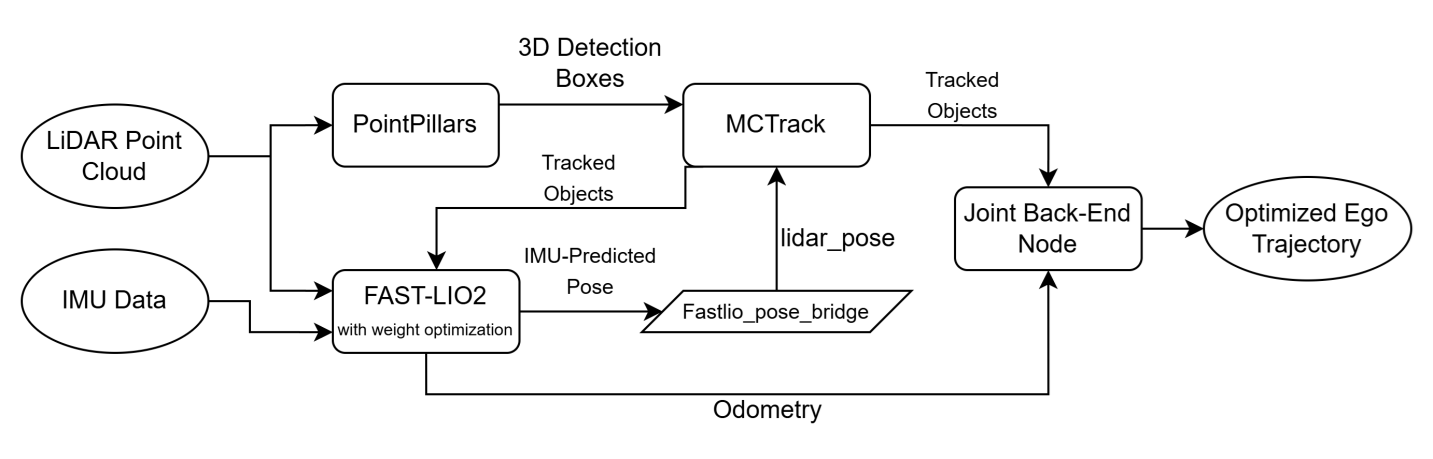
\includegraphics[width=0.96\textwidth]{Overall architecture of the proposed dynamic-scene trajectory optimization framework.png}
    \caption{Overall system architecture. It can be read as a three-layer data flow of localization backbone, object-observation module, and exploratory backend.}
    \label{fig:overall_architecture}
\end{figure}

Figure~\ref{fig:overall_architecture} is easier to read as a data-dependency graph than as a static block diagram. The first layer is the main localization backbone: FAST-LIO estimates ego pose directly from raw LiDAR and IMU measurements. The second layer is the object-level dynamic-observation module: PointPillars publishes 3D detections from the same LiDAR input, \code{fastlio_pose_bridge.py} converts FAST-LIO odometry into the LiDAR-pose interface expected by MCTrack, and MCTrack aligns poses with detections to form coherent object trajectories. The third layer is the localization-enhancement path: tracked objects are fed back to FAST-LIO for dynamic-point down-weighting and forwarded to the ego-only backend as an exploratory mechanism for additional ego-trajectory correction.

This organization is necessary because the modules serve different layers of the localization problem. FAST-LIO works on raw geometry and inertial propagation, PointPillars and MCTrack generate object-level dynamic observations, and the backend performs only short-horizon exploratory ego correction. Keeping these stages explicit avoids blocking behavior and makes it easier to trace localization gains and failures to a specific interface.

If the system is understood from the data-flow perspective, the process can be summarized in seven steps:
\begin{enumerate}[leftmargin=2.2em]
    \item Sensors first acquire raw LiDAR point clouds and IMU data, and feed them simultaneously to FAST-LIO and PointPillars.
    \item PointPillars produces the 3D detections of the current frame, indicating which targets are present nearby.
    \item FAST-LIO outputs the current ego pose and continuously provides higher-frequency motion predictions.
    \item The pose bridge converts these localization outputs into the format directly consumable by the tracking module.
    \item MCTrack combines ``what was observed'' with ``how the ego vehicle moved'' to complete object association, trajectory updates, and velocity estimation.
    \item Tracking outputs are fed back to FAST-LIO so that points likely belonging to dynamic objects can be down-weighted.
    \item The same tracking outputs are also sent to the joint backend to further refine the ego trajectory.
\end{enumerate}

This seven-step description already shows why the system must be organized as a directed but delayed loop. Tracks cannot exist before detections are associated, and dynamic-point weighting cannot be computed before a tracked-object message exists. The track state produced at time \(t\) therefore influences a later scan rather than the same scan. That one-frame delay is not a bug; it is what keeps the loop online without circular blocking.

\subsection{FAST-LIO Front-End}
\begin{figure}[H]
    \centering
    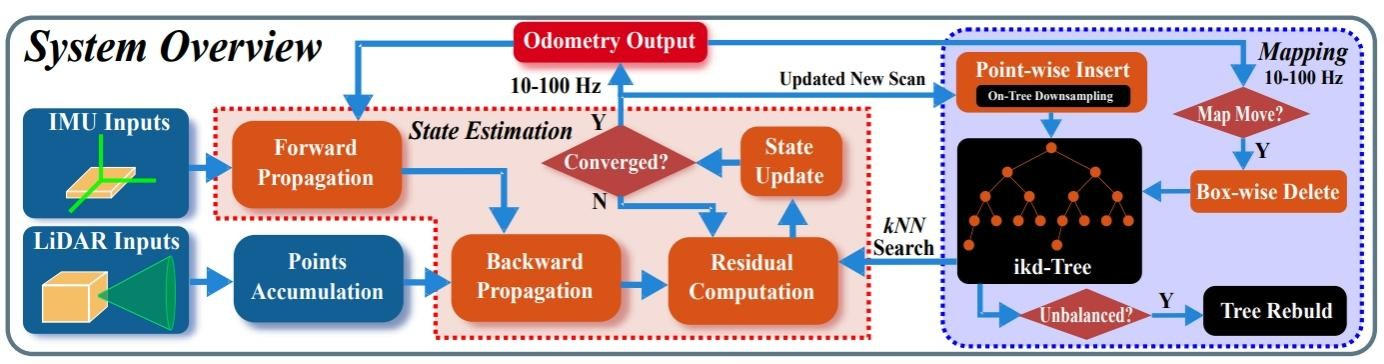
\includegraphics[width=0.82\textwidth]{FAST-LIO2 System Architecture.jpg}
    \caption{FAST-LIO2 front-end architecture, reprinted from Xu \textit{et al.}~\cite{fastlio2}. In this project, object information from MCTrack is injected into the point-cloud preprocessing pipeline to realize adaptive down-weighting of dynamic points.}
    \label{fig:fastlio_architecture}
\end{figure}

FAST-LIO is the localization backbone of the entire system and the starting point of the data flow described above. It directly consumes LiDAR point clouds and IMU data from the KITTI rosbag and internally uses a tightly coupled LiDAR-inertial estimation pipeline to output stable ego poses. In this project, FAST-LIO not only generates globally consistent \code{/Odometry}, but also publishes \code{/Odometry_imu_predicted} as a high-frequency predicted pose, providing a unified reference for later tracking and backend optimization.

From the perspective of module responsibilities, FAST-LIO plays three roles in the system. First, it provides MCTrack with reliable ego poses, allowing 3D detections to be compensated for ego motion before cross-frame association. Second, it supplies the joint backend with raw odometry constraints so that backend optimization does not drift too far from the front-end estimate. Third, through \code{preprocess.cpp} and the tracked-object callback path in \code{laserMapping.cpp}, it receives \code{/mctrack/tracked_objects}, converts them into internal \texttt{DynamicObject} structures, and maps target motion attributes into point-level weights. FAST-LIO therefore acts both as the source of ego-motion information and as the place where object feedback most directly changes scan-level geometry processing.

From an algorithmic viewpoint, the FAST-LIO front-end can be understood as an iterative filter combining IMU propagation with LiDAR geometric correction. Let the system state be \(\mathbf{x}_k\) and the IMU input be \(\mathbf{u}_k\). The prediction step can be written as
\begin{equation}
\mathbf{x}_{k+1|k}=f(\mathbf{x}_{k|k}, \mathbf{u}_k)+\mathbf{w}_k,
\qquad
\mathbf{P}_{k+1|k}=\mathbf{F}_k \mathbf{P}_{k|k}\mathbf{F}_k^\top+\mathbf{Q}_k,
\end{equation}
where \(\mathbf{P}\) is the state covariance and \(\mathbf{F}_k\) is the linearized state-transition matrix. For the \(j\)-th point in the current frame, FAST-LIO further constructs a point-to-plane geometric residual using a reference plane in the local map:
\begin{equation}
r_j=\mathbf{n}_j^\top\!\bigl(\mathbf{R}(\mathbf{x})\,\mathbf{p}_j+\mathbf{t}(\mathbf{x})-\mathbf{q}_j\bigr),
\end{equation}
and minimizes through iterative updates
\begin{equation}
\delta \mathbf{x}^{\star}
=
\arg\min_{\delta \mathbf{x}}
\left(
\sum_{j} \|r_j\|^2_{\mathbf{\Sigma}_j^{-1}}
+\;
\|\delta \mathbf{x}\|^2_{\mathbf{P}_{k+1|k}^{-1}}
\right).
\end{equation}
These equations describe the core role of FAST-LIO in this project. The IMU provides high-frequency continuous prediction, while LiDAR point-cloud residuals pull the pose back toward a geometrically consistent solution. This is why FAST-LIO can not only stably output \code{/Odometry}, but also serve as the spatiotemporal reference for MCTrack.

To feed FAST-LIO outputs into the tracking module, the project implements \code{fastlio_pose_bridge.py}, which converts \code{/Odometry} into \code{/mctrack/lidar_pose} using the configured body-to-LiDAR extrinsic transform and publishes the result as TF. This explicit bridge keeps localization, tracking, and visualization in the same frame convention. FAST-LIO then freezes the latest tracked objects into a scan-local snapshot before preprocessing each scan, so every point is weighted against a consistent object set rather than a mid-scan message buffer.

\subsection{PointPillars Object-Observation Module}
The project integrates the PointPillars detector~\cite{pointpillars} as a ROS node implemented in \path{MMDET3D/local/ros/nodes/kitti_pointpillars_bag_node.py}, allowing it to consume KITTI point clouds directly from rosbag. Its role is not merely to emit raw detections; it provides the localization-enhancement pipeline with unified, traceable, and time-stamped 3D object-observation messages. The project-defined message types in \path{catkin_ws/src/ME5400/msg/Detection3D.msg} and \path{catkin_ws/src/ME5400/msg/Detection3DArray.msg} include frame ID, category, confidence, 2D box, 3D dimensions, LiDAR-frame position, and yaw angle. As a result, PointPillars and MCTrack communicate through explicit project-owned interfaces rather than private third-party message formats.

\begin{figure}[H]
    \centering
    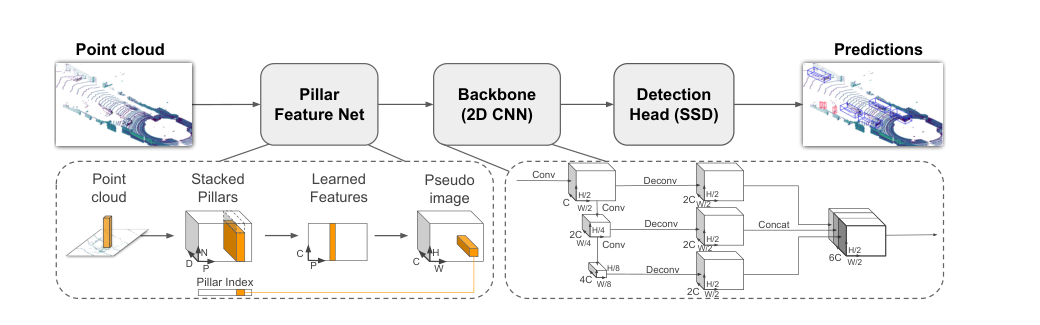
\includegraphics[width=0.95\textwidth]{PointPillars Network Architecture.png}
    \caption{Network architecture from the original PointPillars paper. The network consists of a Pillar Feature Net, a 2D CNN backbone, and an SSD detection head. The image is reproduced from the CVPR 2019 paper by Lang \textit{et al.}~\cite{pointpillars}.}
    \label{fig:pointpillars_architecture}
\end{figure}

The essence of PointPillars is to convert sparse 3D point clouds into a BEV pseudo-image by encoding vertical pillars and then applying a 2D CNN detection head. This transforms a costly 3D convolution problem into a cheaper 2D one, which is exactly why PointPillars fits the real-time requirements of the current online system.

Written in equations, if the \(l\)-th pillar contains the point set \(\mathcal{P}_l=\{\mathbf{p}_i\}\), PointPillars first constructs an augmented feature for each point:
\begin{equation}
\tilde{\mathbf{p}}_i=
\bigl[
x_i,\; y_i,\; z_i,\; r_i,\;
x_i-\bar{x}_l,\; y_i-\bar{y}_l,\; z_i-\bar{z}_l,\;
x_i-x_l^c,\; y_i-y_l^c
\bigr],
\end{equation}
where \((\bar{x}_l,\bar{y}_l,\bar{z}_l)\) is the mean of points inside the pillar and \((x_l^c,y_l^c)\) is the pillar center. After the Pillar Feature Net, the pillar-level feature can be written as
\begin{equation}
\mathbf{f}_l=\max_{i\in \mathcal{P}_l}\phi(\tilde{\mathbf{p}}_i),
\end{equation}
which is then scattered into the BEV pseudo-image:
\begin{equation}
\mathbf{I}(u,v)=
\begin{cases}
\mathbf{f}_l, & (u,v)=\mathrm{index}(l),\\
\mathbf{0}, & \text{otherwise},
\end{cases}
\end{equation}
Finally, the detection head jointly optimizes classification, box regression, and orientation prediction:
\begin{equation}
\mathcal{L}_{\mathrm{det}}
=
\beta_{\mathrm{cls}}\mathcal{L}_{\mathrm{cls}}
+\beta_{\mathrm{loc}}\mathcal{L}_{\mathrm{loc}}
+\beta_{\mathrm{dir}}\mathcal{L}_{\mathrm{dir}}.
\end{equation}
This also explains why PointPillars fits the project well: efficient 2D convolutions are sufficient to produce time-stamped 3D detections for online ROS publishing.

From an engineering perspective, this design serves three purposes. It preserves calibration consistency, keeps a relatively low detection threshold so that pruning happens later through tracking and gating, and exposes a project-defined message contract that can be reused by MCTrack, visualization, evaluation, and replay. PointPillars deliberately does \emph{not} solve tracking internally; its job is to publish geometrically meaningful 3D hypotheses with timestamps and confidence scores so that the downstream system can focus on how those object cues serve localization.

\subsection{MCTrack Object-State Estimation Module and Data-Flow Details}
\begin{figure}[H]
    \centering
    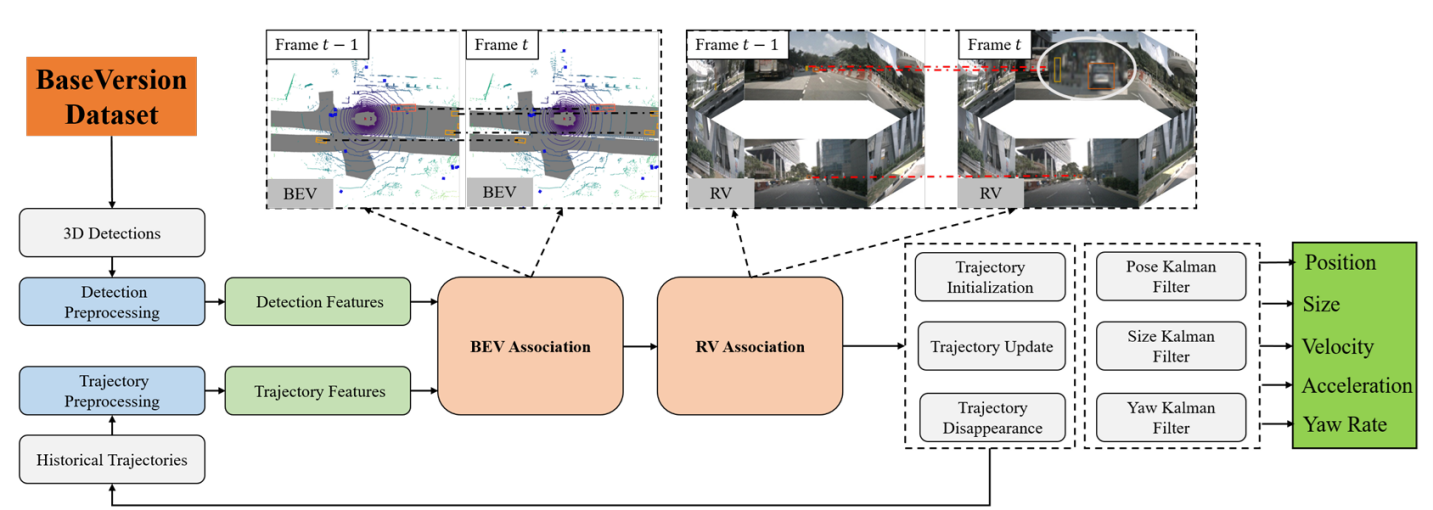
\includegraphics[width=0.92\textwidth]{Overview of 3D MOT framework MCTrack.png}
    \caption{Schematic of the MCTrack 3D MOT framework, reprinted from Wang \textit{et al.}~\cite{mctrack}. Its outputs contain not only position and size, but also velocity, acceleration, trajectory length, and related motion attributes.}
    \label{fig:mctrack_framework}
\end{figure}

The online MCTrack~\cite{mctrack} node is implemented in \code{catkin_ws/src/ME5400/scripts/mctrack_online_node.py}. It subscribes by default to \code{/mctrack/lidar_pose} and \code{/detection/lidar_detections}, maintains an internal pose buffer and a queue of pending detections, and processes detections only after a pose with a suitable timestamp is available. This ``detections wait for pose, pose drives processing'' design avoids the temporal misalignment that arises when messages are processed strictly in order of arrival.

MCTrack publishes both \code{/mctrack/markers} for visualization and \code{/mctrack/tracked_objects} for downstream optimization. In \code{TrackedObject.msg}, in addition to object pose and size, the message records \code{track_length}, \code{velocity}, \code{velocity_fusion}, \code{velocity_diff}, \code{velocity_curve}, and \code{acceleration}. These fields are crucial to this project because the subsequent dynamic-weight optimization and joint-backend gating depend on motion attributes rather than only on box position.

Under the current \texttt{kitti\_fastlio.yaml} configuration, the main state estimate of MCTrack in online mode can be approximated as a 2D constant-velocity Kalman filter. If the trajectory state is
\begin{equation}
\mathbf{x}_k=[p_x,\; p_y,\; v_x,\; v_y]^\top,
\end{equation}
its prediction model is
\begin{equation}
\mathbf{x}_{k|k-1}=
\begin{bmatrix}
1 & 0 & \Delta t & 0\\
0 & 1 & 0 & \Delta t\\
0 & 0 & 1 & 0\\
0 & 0 & 0 & 1
\end{bmatrix}
\mathbf{x}_{k-1|k-1},
\qquad
\mathbf{H}=
\begin{bmatrix}
1 & 0 & 0 & 0\\
0 & 1 & 0 & 0
\end{bmatrix},
\qquad
\mathbf{z}_k=\mathbf{H}\mathbf{x}_{k|k-1}+\mathbf{v}_k,
\end{equation}
followed by the standard Kalman update
\begin{equation}
\mathbf{K}_k=\mathbf{P}_{k|k-1}\mathbf{H}^\top(\mathbf{H}\mathbf{P}_{k|k-1}\mathbf{H}^\top+\mathbf{R})^{-1},
\qquad
\mathbf{x}_{k|k}=\mathbf{x}_{k|k-1}+\mathbf{K}_k(\mathbf{z}_k-\mathbf{H}\mathbf{x}_{k|k-1}).
\end{equation}
At the data-association level, the current online configuration mainly uses a 3D cost matrix based on predicted boxes together with Hungarian matching:
\begin{equation}
\mathcal{A}^{\star}
=
\arg\min_{\mathcal{A}\in\Pi}
\sum_{(i,j)\in\mathcal{A}} C_{ij},
\qquad
C_{ij}=1-\mathrm{RO\mbox{-}GDIOU}_{3D}\!\left(\hat{B}_i,\; B_j\right),
\end{equation}
where \(\hat{B}_i\) is the predicted track box and \(B_j\) is the current detection box. In other words, FAST-LIO first stabilizes the cross-frame geometry through ego pose, after which MCTrack converts discrete detections into continuous trajectories through motion prediction and global optimal matching. This is the foundation on which later velocity estimation, dynamic weights, and the joint backend become possible.

The buffering and timestamp logic are particularly important. MCTrack stores a finite \texttt{pose\_buffer} and a queue of pending detections. For each detection message, it looks for poses immediately before and after the detection timestamp; if both exist, it interpolates, otherwise it waits briefly and then falls back to the nearest available pose. This is a practical compromise between strict synchronization and online liveness. MCTrack also preserves both world-frame \texttt{pose} and LiDAR-frame \texttt{lidar\_pose}, because FAST-LIO needs the LiDAR-frame version for point-box intersection while the backend compares propagated world-frame object motion against the ego state.

Seen this way, PointPillars and MCTrack are not merely a detector and a tracker within the system. Together they form the dynamic-observation path that provides object-level geometry and motion semantics to the localization modules. FAST-LIO provides the stable ego reference, PointPillars provides time-stamped object hypotheses, and MCTrack turns those hypotheses into track states that can be propagated over time. Only after this transformation does dynamic weighting or object-consistency residual design become meaningful for localization enhancement.

\subsection{Temporal Alignment, Coordinate Frames, and Failure Modes}
In the optimized online run, rosbag playback publishes only raw LiDAR and IMU topics, while PointPillars, FAST-LIO, MCTrack, and the backend run as separate ROS nodes with different callback timings. Time synchronization is therefore a runtime issue rather than a one-time calibration issue, which is why the pose buffer, pending-detection queue, and one-frame delayed weighting loop are structural parts of the architecture.

The main runtime failure modes are straightforward: \textbf{detection latency} forces the tracker to use a nearby rather than truly synchronized pose; \textbf{missed detections} shorten tracks and destabilize motion estimates; \textbf{track fragmentation} destroys the continuity needed for weighting and backend reuse; and \textbf{timestamp or frame inconsistency} can magnify velocity-extrapolation error or even turn an interface bug into an apparent algorithmic failure. The architecture reduces these risks, but does not eliminate them.

\section{Engineering Implementation and System Integration}
\subsection{Overall Code Organization}
The repository layout is intentionally organized around integration responsibility rather than around algorithm names alone. The top-level directories that matter most to this report are \texttt{catkin\_ws/}, \texttt{MCTrack/}, \texttt{MMDET3D/}, \texttt{Scripts/}, and \texttt{Results/}. \texttt{catkin\_ws/} contains the ROS-native part of the system: custom messages, launchable scripts, configuration files, and the modified FAST-LIO package. \texttt{MCTrack/} preserves the tracking framework and configuration in a relatively self-contained form so that the online node can import and wrap it rather than reimplementing tracking logic. \texttt{MMDET3D/} contains the detector-side code used to wrap PointPillars into the ROS pipeline. \texttt{Scripts/} contains orchestration logic, helper utilities, and one-click entry points. \texttt{Results/} is not a passive dump folder; it is the standardized experiment archive that the report depends on for every figure and metric.

This partition is beneficial for two reasons. First, it separates heavy third-party or framework-dependent code from project-specific integration code. That makes it easier to upgrade one module without destabilizing all others. Second, it maps closely to the user's actual workflow. During experimentation, the user rarely edits a detector kernel or Kalman update directly; instead, the user launches scripts, checks logs, inspects ROS topics, records trajectories, and compares result folders. Organizing the repository to match that workflow reduces friction and shortens the feedback cycle during debugging and evaluation. The public course-project repository is \url{https://github.com/XC-CN/ME5400}, and the report's script names, result paths, and engineering descriptions refer to that codebase.

\begin{table}[H]
    \centering
    \caption{Representative entry scripts of the online system and their functions}
    \label{tab:code_design}
    \footnotesize
    \begin{tabularx}{\textwidth}{L{2.4cm} L{5.3cm} Y}
        \toprule
        Module & Representative entry scripts & Function summary \\
        \midrule
        Online baseline &
        \makecell[tl]{\code{run_baseline.sh}\\\code{run_fastlio.sh}} &
        Executes the pure FAST-LIO online baseline pipeline and records the baseline trajectory in \code{trajectory_baseline.txt}. \\
        Online optimization &
        \makecell[tl]{\code{run_optimized.sh}\\\code{run_pointpillars_node.sh}\\\code{run_mctrack_online_node.sh}\\\code{run_joint_backend_ego.sh}} &
        Orchestrates PointPillars, MCTrack, dynamic-weight FAST-LIO, and the joint backend, and outputs the optimized front-end trajectory \code{trajectory.txt} together with the backend trajectory \code{trajectory_joint.txt}. \\
        One-click online comparison & \code{run_all.sh} & Sequentially runs the online baseline and online optimization pipelines and archives the complete runtime logs into the result directory. \\
        Evaluation and archiving &
        \makecell[tl]{\code{evaluate_trajectories.py}\\\code{odom_to_tum_recorder.py}} &
        Uniformly generates quantitative metrics and visualization files, including \code{metrics.json}, trajectory-error comparison plots, and summary figures. \\
        \bottomrule
    \end{tabularx}
\end{table}

\begin{table}[H]
    \centering
    \caption{Main repository directories and their engineering roles}
    \label{tab:repo_layout}
    \footnotesize
    \begin{tabularx}{\textwidth}{L{2.3cm} L{4.2cm} Y}
        \toprule
        Directory & Representative contents & Engineering role \\
        \midrule
        \code{catkin_ws/} & \makecell[tl]{\code{src/ME5400/msg/}\\\code{src/ME5400/scripts/}\\\code{src/fast_lio/}} & ROS-native workspace for custom interfaces, bridge nodes, MCTrack online wrapper, joint backend, trajectory recording, and the modified FAST-LIO front-end. \\
        \code{MCTrack/} & \code{config/kitti_fastlio.yaml}, tracker modules & Encapsulates the tracking framework and motion/association configuration used by the online ROS node. \\
        \code{MMDET3D/} & PointPillars ROS wrapper and detector utilities & Hosts the detector-side code needed to run PointPillars in the project's data and topic conventions. \\
        \code{Scripts/} & \makecell[tl]{\code{run_all.sh}\\\code{run_baseline.sh}\\\code{run_optimized.sh}\\\code{evaluation/}} & Provides one-click execution, build/setup helpers, evaluation entry points, and the scripted experiment workflow. \\
        \code{Results/} & \code{metrics.json}, trajectories, plots, logs & Serves as the canonical archive for sequence-level outputs used in later analysis, report writing, and regression checking. \\
        \bottomrule
    \end{tabularx}
\end{table}

\subsection{Online System Design}
In online mode, \code{run_all.sh} sequentially executes \code{run_baseline.sh} and \code{run_optimized.sh}. This is not just a convenience wrapper. It encodes the fairness policy of the experiments. The baseline run launches only \code{roscore}, FAST-LIO, and rosbag playback so that a pure localization trajectory is recorded as \code{trajectory_baseline.txt}. The optimized run then launches PointPillars, MCTrack, FAST-LIO in \texttt{both} mode, and the joint backend, while \code{odom_to_tum_recorder.py} records \code{/joint_backend/odom} into \code{trajectory_joint.txt}. Because the scripts operate on the same sequence ID, use the same data source, and archive outputs into the same result folder, they provide a controlled comparison rather than a loose collection of independent runs.

The control flow of the online optimization script is also chosen to minimize race conditions. PointPillars starts first because its model initialization is typically the slowest. MCTrack starts next and waits until it is ready to receive poses and detections. FAST-LIO with dynamic weighting is then launched so that the tracker can immediately begin filling its pose buffer once odometry appears. Finally, the joint backend starts and trajectory recording begins. If this order were reversed, several predictable problems would appear: the recorder might start before any backend topic exists; the tracker might begin queuing detections without usable poses; or the detector might publish too late, causing a burst of stale detections. Figure~\ref{fig:online_sequence_logic} therefore documents more than a conceptual loop; it records the actual execution logic that keeps the optimized chain stable.

\begin{figure}[htbp]
    \centering
    \resizebox{0.98\textwidth}{!}{\onlineSequenceFigure}
    \caption{Execution-level temporal logic of the online optimization chain. When FAST-LIO processes the current LiDAR frame, it uses the frozen \texttt{tracked\_objects} snapshot from the previous frame. The tracking result produced by MCTrack at the current frame mainly enters the dynamic down-weighting chain in the next frame.}
    \label{fig:online_sequence_logic}
\end{figure}

As Figure~\ref{fig:online_sequence_logic} shows, the online chain is not a synchronous loop in which the current-frame detections immediately modify the current-frame point cloud. Instead, it is an asynchronous loop with a one-frame delay. During \code{preprocess()}, FAST-LIO first freezes the previous \code{/mctrack/tracked_objects} snapshot and softly down-weights points in the current scan that fall inside dynamic boxes. The current \code{/Odometry}(t) is then passed through the bridge to MCTrack, aligned with \code{/detection/lidar_detections}(t) from PointPillars, and used to update object states. The newly produced \code{/mctrack/tracked_objects}(t) is then sent to both FAST-LIO and the joint backend, but its effect on FAST-LIO appears only in the next frame. This design avoids intra-frame blocking, limits lock contention inside the preprocessor, and explains why the current system can form a front-end closed loop while remaining runnable online.

After rosbag playback finishes, the script archives \code{trajectory.txt}, \code{trajectory_joint.txt}, logs, and evaluation plots into \code{Results/<seq>_results/Online/}. The benefit of this design is not just cleanliness. It allows a later report or debugging pass to reconstruct exactly what happened for a given sequence: which scripts ran, which trajectories were compared, what the metrics were, and how the front-end and backend plots looked. The limitation, of course, is that the system is still loosely coupled at the topic level: modules share messages rather than a unified graph state. But from an engineering perspective, explicit message passing is precisely what makes the current prototype inspectable and rerunnable within the current project workflow.

\subsection{Result Archiving and the Scripted Experimental Pipeline}
The result archive under \code{Results/<seq>_results/Online/} is best understood as a formal experiment contract. Every online sequence folder contains the baseline trajectory, the optimized front-end trajectory, the joint-backend trajectory when available, a plain-text report, a JSON report, comparison plots, and a full runtime log. This means that quantitative analysis in the report does not depend on manually copied numbers or ephemeral terminal output. It depends on versioned artifacts that can be regenerated by rerunning the scripts within the same repository workflow. In this report, that is the operative meaning of repeatability: the same scripted pipeline can be rerun and the same categories of metrics, plots, and logs can be recovered under the current project setup, without claiming machine-independent byte-identical reproduction. In practice, this is what makes later section-level expansion possible: ATE, RPE, Tr, Rot, failure sequences, and plots all originate from the same archived source.

The evaluation path reinforces this repeatability goal. \code{evaluate_trajectories.py} loads the recorded TUM trajectories, associates them with KITTI ground truth, computes ATE and RPE, aligns trajectories for visualization, and computes KITTI-style relative translation and rotation metrics when enough matched path length exists. Because the same script is used for every baseline versus optimized comparison, the report avoids a common course-project weakness in which each sequence is evaluated slightly differently. Even when different sequences expose different available span lengths, as in short versus long trajectories, the evaluation rule is still consistent.

This workflow-level repeatability is not a secondary convenience; it is part of the intellectual contribution of the project. A course project that claims a localization gain but cannot rerun its own sequences, recover its own metrics, or explain its own failures has limited value. By contrast, the present system can be launched with fixed scripts, can record trajectories in a standard format, can regenerate figures, and can tie every conclusion in the report back to a concrete archived artifact. That is why engineering repeatability within the repository workflow deserves to be treated as a first-class outcome rather than an appendix-level detail.

\subsection{ROS Topics, Message Interfaces, and Integration Difficulties}
The module boundaries in this repository are enforced primarily through ROS topics and project-defined messages. The raw inputs are \code{/kitti/velo/pointcloud} and \code{/kitti/oxts/imu}. FAST-LIO publishes \code{/Odometry} and \code{/Odometry_imu_predicted}. The bridge node republishes \code{/mctrack/lidar_pose}. PointPillars publishes \code{/detection/lidar_detections}. MCTrack publishes \code{/mctrack/tracked_objects} and \code{/mctrack/markers}. The backend publishes \code{/joint_backend/odom}. Each topic corresponds to a clear semantic responsibility, and the custom message definitions ensure that detector outputs, tracked-object states, and backend inputs remain interpretable throughout the pipeline.

The custom messages are especially useful for avoiding hidden coupling. \code{Detection3D.msg} stores frame index, class, confidence, 2D box, 3D dimensions, LiDAR-frame location, and yaw. \code{TrackedObject.msg} extends that into an object state useful for feedback, including track length, world-frame pose, LiDAR-frame pose, fused velocity, velocity difference, curved velocity, and acceleration. This explicitness is what makes the dynamic-weight module and backend feasible. The weighting code can read LiDAR-frame pose, track length, score, and acceleration directly. The backend can compare local observations to world-frame predictions without trying to reconstruct state from an opaque tracker object. In short, the message layer is where the project translates algorithm-specific internals into stable cross-module contracts.

The integration was still difficult in several ways. Dependency isolation is one challenge: MMDET3D, ROS, MCTrack, and FAST-LIO each bring their own runtime assumptions, environment variables, and build expectations. Startup order is another challenge, because the whole optimized pipeline is sensitive to whether detector, tracker, and backend are ready before rosbag playback begins. Logging is a third challenge, addressed by redirecting full script output to per-sequence logs. Result naming and archival are a fourth challenge: if trajectory files were not renamed and moved consistently, later evaluation would silently compare the wrong outputs. These are mundane issues individually, but together they determine whether an integrated robotics system behaves like a controlled experiment or like an unstable demo.

\section{Dynamic Weight Optimization}
\subsection{Design Motivation and Code Location}
The central design question of this module is simple: when a tracked object overlaps a region of the point cloud, should the system keep those points, remove them, or reduce their influence continuously? The current project chooses the third option. Instead of turning dynamic-point handling into a binary segmentation problem, it treats tracked objects as evidence that the reliability of nearby geometry should be reduced by a degree that depends on motion state and confidence. This is motivated by both geometry and engineering. Geometrically, hard removal can erase too much useful structure in traffic scenes where large vehicles occupy a significant share of the scan and where roadside geometry may already be sparse. Engineering-wise, hard removal is brittle under false positives, unstable boxes, and partial occlusion; a slightly wrong box can delete a large amount of valid structure. Soft weighting is more conservative and therefore more appropriate for a first integrated prototype.

The current implementation lives mainly in \code{catkin_ws/src/fast_lio/src/preprocess.cpp}, with tracked-object conversion in \code{catkin_ws/src/fast_lio/src/laserMapping.cpp}. After FAST-LIO receives \code{/mctrack/tracked_objects}, each object is converted into an internal \texttt{DynamicObject} that stores its LiDAR-frame center, bounding-box half-sizes, local yaw representation, timestamp, and a scalar weight. Importantly, the conversion uses the object's LiDAR-frame pose rather than its world-frame pose, because point-in-box tests must be carried out in the current LiDAR coordinate system. This makes the weighting stage tightly tied to actual preprocessing rather than to some abstract global map representation.

Compared with earlier versions, the default parameters for dynamic weighting in the current code are explicitly fixed as follows:
\begin{itemize}[leftmargin=2em]
    \item reference velocity \(\,v_{\mathrm{ref}}=10.0\);
    \item reference acceleration \(\,a_{\mathrm{ref}}=4.0\);
    \item velocity penalty coefficient \(\alpha_v=0.5\);
    \item acceleration penalty coefficient \(\alpha_a=0.3\);
    \item detection-score penalty coefficient \(\alpha_s=0.2\);
    \item minimum weight \(w_{\min}=0.2\);
    \item bounding-box margin \(xy=0.5\,\mathrm{m},\,z=0.5\,\mathrm{m}\);
    \item object timeout \(1.0\,\mathrm{s}\), with a minimum trajectory-length threshold of 3.
\end{itemize}

Each parameter reflects an engineering compromise. The reference velocity and acceleration define what should count as clearly dynamic, the minimum weight prevents the scheme from collapsing into hard deletion, the box margin compensates for imperfect boundaries, and the timeout plus minimum track length prevent stale or immature trajectories from influencing the scan.

\subsection{Weight Computation}
Suppose that a tracked target has velocity \(v\), acceleration \(a\), and detection score \(s\). The code first normalizes these quantities:
\begin{equation}
\hat{v}=\mathrm{clamp}\!\left(\frac{v}{v_{\mathrm{ref}}}\right), \qquad
\hat{a}=\mathrm{clamp}\!\left(\frac{a}{a_{\mathrm{ref}}}\right), \qquad
\hat{s}=\mathrm{clamp}(s).
\end{equation}
It then constructs the penalty term
\begin{equation}
p = \alpha_v \hat{v} + \alpha_a \hat{a} + \alpha_s \hat{s},
\end{equation}
and computes the dynamic weight as
\begin{equation}
w = \mathrm{clip}(1-p,\; w_{\min},\; 1).
\end{equation}

The resulting interpretation is intuitive. Faster targets with larger acceleration and higher detection score receive smaller point weights. If a trajectory is short, nearly static, or weakly scored, the system preserves a larger weight. The trajectory-length guard is particularly important: if \texttt{track\_length} is below threshold, \texttt{weightFromAttributes()} returns \(1.0\), so the object cannot influence the point cloud yet.

The choice of velocity, acceleration, and score reflects the information the tracker can already provide reliably. This is not a fully probabilistic uncertainty model, but it is a practical heuristic built from interpretable motion attributes already present in \texttt{TrackedObject.msg}.

\subsection{From Tracked Objects to Point-Level Weights}
The transformation from object tracks to point weights happens in one scan-local pipeline. The tracked-object callback converts each object into an internal representation using \code{lidar_pose.position}, margin-expanded half sizes, a compact yaw representation, and a scalar weight computed from fused speed, acceleration, detection score, and track length. When a new scan enters \code{process()}, FAST-LIO freezes the latest tracked objects into an active snapshot. Each point then calls \code{computePointWeight()}, checks whether it lies inside any non-expired dynamic box, and takes the minimum weight among the boxes that cover it. This means \code{tracked_objects}(t) does not retroactively modify the scan at time \(t\); it becomes the consistent object set used when preprocessing a later scan.

The weight becomes effective directly in point-cloud preprocessing. For each input point, if \texttt{computePointWeight()} finds dynamic-box overlap, the point's \texttt{intensity} is updated to the smaller of the original intensity and the dynamic weight:
\begin{equation}
I'_j = \min(I_j,\; w_j),
\end{equation}
where \(I_j\) is the original point intensity and \(w_j\) is the computed dynamic weight. This reuses the existing FAST-LIO point representation to carry reliability information downstream without rewriting the registration machinery.

Compared with outright deleting dynamic points, this strategy is more robust to box-boundary error, detection jitter, and partially dynamic regions; it preserves some geometric support when static background is limited; and it differentiates between a clearly moving mature track and a barely confirmed object without a hard semantic switch. This graded behavior is one reason the front-end loop is more stable than the current backend.

\subsection{Boundary Cases and Parameter Sensitivity}
Several boundary cases clarify why soft weighting is preferable in the current system. \textbf{False positives} and \textbf{occlusion-driven box instability} can overlap static structure or jitter in extent; under hard deletion those errors would erase geometry completely, whereas soft weighting only reduces influence and only after track maturity and motion checks pass. \textbf{Temporally uncertain cases}, including temporarily stopped vehicles and stale trajectories, are handled more conservatively through the combination of score, acceleration, minimum track length, and timeout.

Although the project does not include a formal parameter sweep, the archived sequences support a qualitative sensitivity discussion. If \(v_{\mathrm{ref}}\) is too low or \(w_{\min}\) too small, the module behaves too much like hard filtering; if \(v_{\mathrm{ref}}\) is too high or \(w_{\min}\) too large, dynamic weighting becomes too weak to matter. The current values appear to be a practical middle ground: strong enough to help on drift-prone sequences such as 0010 and 0020, but conservative enough to avoid systematic degradation across all seven online runs.

The broader effect is improved scan matching and local-map consistency without demanding that object-derived information already be accurate enough to support strong backend corrections. This balance is why dynamic weighting is the most stable gain source in the current system.

\section{Joint Backend Optimization}
\subsection{The Ego-Only Sliding-Window Problem}
The joint backend is implemented in \code{catkin_ws/src/ME5400/scripts/joint_backend_ego_node.py}, with configuration stored in \code{catkin_ws/src/ME5400/config/joint_backend_ego.yaml}. Its purpose is intentionally transitional. Rather than solving a full object-centric SLAMMOT problem immediately, it tests a narrower hypothesis at manageable engineering cost: can stable tracked objects provide enough additional structure to refine the ego trajectory, even if object states are not jointly optimized? The answer matters because it determines whether the project should invest later effort in a richer backend at all. An ego-only backend is therefore not the final goal; it is a diagnostic stepping stone.

The current configuration makes this compromise explicit. The default window length is 8 frames. The object-factor coefficient is \(\lambda_{\mathrm{obj}}=0.12\). The score threshold is 0.6, the track-length threshold is 5, the maximum allowed timestamp difference is 0.1\,s, and the maximum allowed velocity jump is 2.0\,m/s. The minimum object weight is 0.03. The backend uses a Huber robust loss with scale 0.5, optimizes at 10 Hz, and falls back to \([0.20, 0.20, 0.10]\) if the incoming FAST-LIO covariance is invalid. None of these choices is arbitrary. Together they define a backend that is intentionally conservative about when to trust object information and intentionally lightweight about how much state to optimize.

The optimization variable for each frame in the window is written as
\begin{equation}
\mathbf{p}_i=[x_i, y_i, \psi_i]^\top,
\end{equation}
meaning that only planar position and yaw are retained per frame. This choice is restrictive, but it is reasonable for two engineering reasons. First, the tracked-object information used by the backend is already mostly 2D in its motion semantics: fused velocities and association stability are primarily meaningful in the ground plane. Second, retaining only the most critical ego variables keeps the optimization small enough that it can run repeatedly online without becoming the dominant compute bottleneck. The obvious trade-off is that object errors cannot be jointly estimated and can only be used as external observations; if a track is wrong, the backend has no internal variable representing that object's state to absorb the error.

Choosing this ego-only formulation first was therefore a deliberate risk-control strategy. A full joint graph would have required object poses, velocities, data-association uncertainty, marginalization policy, and probably more careful motion-model design. By contrast, the current backend can be implemented, tested, and stress-analyzed using information already produced by MCTrack. This is why it is best described as a prototype of the backend direction rather than as the backend solution itself.

\subsection{Residual Modeling and the Gating Strategy}
The joint backend includes two major residual types. The first is odometry-consistency residuals: relative poses between adjacent FAST-LIO frames are treated as the primary constraints of the sliding window, ensuring that optimization does not deviate excessively from the original odometry. The second is object-observation consistency residuals: for each frame, the backend matches the nearest tracking snapshot in time and retains only objects that satisfy score, track-length, velocity-jump, and time-synchronization gates. For each retained object, the code first extrapolates its world-coordinate position to the current frame timestamp using its velocity and then projects it into the ego local frame used during optimization, yielding the predicted observation \(z^{\mathrm{pred}}_{ik}\). The measured observation \(z^{\mathrm{meas}}_{ik}\) comes from the LiDAR-local pose stored in \texttt{TrackedObject}. The object residual is therefore
\begin{equation}
r^{\mathrm{obj}}_{ik}=z^{\mathrm{pred}}_{ik}-z^{\mathrm{meas}}_{ik}.
\end{equation}

The overall optimization objective is
\begin{equation}
\min_{\{\mathbf{p}_i\}}
\sum_{i=2}^{N}\|r^{\mathrm{odom}}_i\|_{W_i}^2
\;+\;
\sum_{i=1}^{N}\sum_{k\in\mathcal{V}_i}
w_{ik}\,\rho\!\left(\|r^{\mathrm{obj}}_{ik}\|_2^2\right),
\end{equation}
where \(\rho(\cdot)\) is a Huber or Cauchy robust kernel and \(\mathcal{V}_i\) denotes the set of objects that pass the gates. In the current code, the object-factor weight is approximately written as
\begin{equation}
w_{ik}=
\max\!\Bigl(
w_{\min}^{\mathrm{obj}},
\sqrt{\lambda_{\mathrm{obj}}}\cdot
(0.5\,\hat{s}_{ik}+0.5\,\hat{\ell}_{ik})
\Bigr),
\end{equation}
that is, it is jointly determined by normalized score and normalized trajectory length.

This residual structure is intentionally asymmetric. The odometry residuals are treated as the stable backbone of the window. The object residuals act as optional corrections whose role is to nudge the solution when object evidence is mature and consistent. The backend therefore does not ask tracked objects to dominate the estimate. It asks them to provide a secondary source of agreement about how the ego platform should be situated relative to the observed scene. That asymmetry is sensible for a prototype, because it limits how much damage a bad track can do. At least in theory, the odometry chain should still anchor the window even when some object factors are imperfect.

In practice, the gating strategy determines whether this theory holds. The backend first discards any track whose score is below threshold, whose track length is too short, whose velocity jump exceeds the allowed maximum, or whose timestamp differs too much from the current odometry state. These conditions correspond closely to the actual failure channels of tracked-object reuse. Low score suggests uncertain detection quality. Short track length suggests immature temporal evidence. Large velocity jumps often indicate a track update that is numerically unstable or semantically wrong. Excessive timestamp mismatch makes velocity extrapolation unreliable even if the track itself is good. The gating policy is therefore not arbitrary conservatism. It is the encoded belief about which tracked objects are mature enough to be treated as weak moving anchors for the ego state.

\subsection{Window Update Logic and Practical Behavior}
The backend is driven by a timer callback rather than by optimization on every message. It stores recent odometry states and track snapshots in ring buffers, builds the latest window when enough frames exist, and avoids re-optimizing the same window end stamp. The optimized result is applied as a correction to the latest raw odometry pose, preserving FAST-LIO roll and pitch while adjusting planar position and yaw. The backend therefore behaves more like an online corrector than a full smoothing engine.

This explains the mixed experimental behavior observed later. When object information is clean and baseline drift is significant, the backend can provide useful low-frequency correction. When object information is noisy, a few bad residuals can remain visible because the window is small and object states are not jointly estimated.

\subsection{Value and Limitations of the Joint Backend}
The engineering value of this backend is that it validates a key proposition: even when object states are not treated as explicit optimization variables, stable tracked objects can still act as temporary moving anchors that impose additional constraints on the ego trajectory. In other words, the system has already moved beyond the view that dynamic targets are merely noise to be filtered out. The backend therefore serves as a proof-of-direction. It shows that tracked objects can enter the estimation problem as positive information, not only as sources of point down-weighting.

Its limitations, however, are equally clear. Because object states come from point estimates of the tracker and are extrapolated through velocity propagation, any noise in object velocity, detection boxes, or association results can be injected back into the ego pose. The backend also lacks richer factor diversity: there are no explicit object-state variables, no stronger confidence model than score and track length, and no sophisticated data-association uncertainty representation. Moreover, the motion model implicit in the tracker is still relatively simple, so extrapolated object positions are not always trustworthy enough to constrain ego motion.

Sequence 0009 is the clearest failure case. In online mode, the baseline ATE RMSE is 1.6831\,m and the front-end loop slightly improves it to 1.6675\,m, but the joint backend degrades the ATE RMSE to 3.3082\,m, while RPE RMSE rises from 0.1787 to 1.9514. The most plausible interpretation is not that object information is useless in principle, but that several weak links aligned negatively in this sequence. Velocity extrapolation likely accumulated error over short object horizons. Timestamp mismatch, even if within the nominal gate, likely reduced the physical meaning of propagated object states. Gating based on score, track length, and velocity jump was not sufficient to suppress all harmful factors. Once those residuals entered a small ego-only window, the optimizer had no object-state variables or stronger uncertainty model to absorb the inconsistency. This makes Sequence 0009 far more convincing as a diagnostic example than a generic statement that the backend is ``sometimes unstable.''

The correct conclusion is therefore measured. The backend direction is valid, because some sequences do show useful drift correction and because the formulation already demonstrates how object information can enter ego optimization. But the present ego-only implementation remains an engineering prototype rather than a robust joint backend. A reasonable evolution path is clear: add better confidence modeling, incorporate object-state variables directly, enrich the factor set beyond simple object observations, and eventually move toward an object-centric backend in which ego motion and object motion are estimated together instead of one being used only as a correction source for the other.

\section{Experimental Analysis}
\subsection{Experimental Setup and Result Sources}
The experiments in this report are uniformly based on the archived online results already stored under \texttt{Results/}. The analyzed online sequences are 0003, 0006, 0007, 0009, 0010, 0013, and 0020. All numerical values are taken from the corresponding \texttt{metrics.json} files, and the discussed plots correspond to \texttt{evaluation\_result.png}, \texttt{evaluation\_joint\_backend.png}, and \texttt{ablation\_bar.png} (summary bar chart). This section therefore does not present new experiments performed during report writing; it consolidates and interprets the experiment artifacts already generated by the archived scripted pipeline.

In online mode, three configurations are compared: \texttt{Baseline}, \texttt{FAST-LIO+MCTrack}, and \texttt{Joint Backend}. The baseline is pure FAST-LIO. \texttt{FAST-LIO+MCTrack} simultaneously introduces pose-assisted tracking and tracking-informed dynamic weighting, while directly evaluating the resulting front-end optimized trajectory. \texttt{Joint Backend} further evaluates the ego-only backend output recorded from \texttt{/joint\_backend/odom}. This ordering is analytically useful because it isolates the effect of the front-end loop from the additional effect, positive or negative, of the backend stage. It should also be stated explicitly that the archived experiments validate the effectiveness of this front-end combination as a whole, rather than providing a strict ablation that cleanly separates ``pose-assisted tracking'' from ``dynamic weighting.'' Accordingly, later statements about the source of front-end gain should be understood as judgments about the combined mechanism, not as a complete causal attribution to any single internal component.

The main evaluation metrics serve different purposes and should not be conflated. \textbf{ATE RMSE} measures the root-mean-square global trajectory deviation after alignment to ground truth, so it is most informative about accumulated drift and overall path consistency. \textbf{RPE RMSE} measures short-horizon relative motion disagreement, so it is more sensitive to local frame-to-frame stability. \textbf{KITTI relative translation error} \(Tr\) summarizes percentage translation error over path segments of fixed length, while \textbf{KITTI relative rotation error} \(Rot\) summarizes angular drift per 100 m. A method can therefore improve ATE without improving RPE, or improve translation consistency without improving rotation consistency. This distinction is important for interpreting the current backend, which sometimes behaves like a coarse drift corrector but not a uniformly better local optimizer.

The seven selected sequences cover a useful range of operating conditions. Sequence 0010 and Sequence 0020 are representative of high-dynamic or drift-prone settings in which front-end feedback has room to show a large gain. Sequences 0003 and 0006 are shorter or more moderate cases in which the front-end improves but the backend can over-correct. Sequences 0007 and 0013 represent relatively stable cases where improvements are limited but generally consistent. Sequence 0009 is the critical failure case in which the backend degrades severely. Organizing the analysis by these scene characteristics is more informative than discussing each sequence as an isolated number.

\begin{figure}[H]
    \centering
    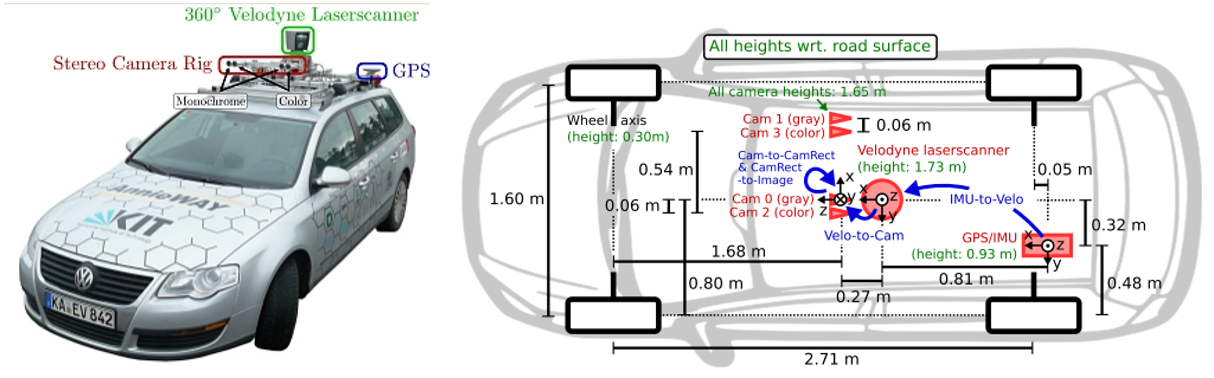
\includegraphics[width=0.62\textwidth]{The KITTI data collection vehicle.png}
    \caption{KITTI data-collection platform, reprinted from benchmark materials associated with Geiger \textit{et al.}~\cite{kitti}. All experiments in this report are based on archived KITTI Tracking results.}
    \label{fig:kitti_vehicle}
\end{figure}

\subsection{Online Experiments: Aggregate Results}
Table~\ref{tab:online_ate} summarizes ATE and RPE for all online sequences. The most important aggregate observation is immediate: \texttt{FAST-LIO+MCTrack} improves ATE RMSE over the baseline on all seven selected online sequences. This 7/7 behavior is stronger evidence than any single large success case because it shows that the front-end loop remains consistently beneficial on this selected evaluation slice. By contrast, \texttt{Joint Backend} further reduces ATE on only four sequences, and two of those gains are effectively neutral in practice. The backend therefore does not exhibit the same cross-sequence stability as the front-end loop, even within this seven-sequence comparison.

\begin{table}[H]
    \centering
    \caption{Summary of online ATE/RPE results. Improvement percentages are computed relative to \texttt{Baseline}; positive values indicate lower error.}
    \label{tab:online_ate}
    \resizebox{\textwidth}{!}{
    \begin{tabular}{ccccccc}
        \toprule
        Sequence & Baseline ATE & F+M ATE & F+M Improvement & Joint ATE & Joint Improvement & RPE RMSE (B/F/J) \\
        \midrule
        0003 & 0.5294 & 0.4513 & +14.75\% & 0.5875 & -10.98\% & 0.2049 / 0.1809 / 0.2393 \\
        0006 & 0.5238 & 0.4710 & +10.09\% & 0.5576 & -6.45\% & 0.1324 / 0.0869 / 0.1677 \\
        0007 & 2.3128 & 2.2393 & +3.18\% & 2.2393 & +3.18\% & 0.1716 / 0.1683 / 0.1683 \\
        0009 & 1.6831 & 1.6675 & +0.93\% & 3.3082 & -96.56\% & 0.1787 / 0.1651 / 1.9514 \\
        0010 & 3.7651 & 0.8680 & +76.95\% & 0.9632 & +74.42\% & 0.2774 / 0.2281 / 0.2334 \\
        0013 & 0.6047 & 0.5816 & +3.82\% & 0.5816 & +3.82\% & 0.1495 / 0.1392 / 0.1392 \\
        0020 & 11.7323 & 6.7938 & +42.09\% & 6.8829 & +41.33\% & 0.2250 / 0.2245 / 0.2270 \\
        \bottomrule
    \end{tabular}}
\end{table}

The ATE table also shows why the backend should not be judged only by average improvement. Sequence 0010 is a major success for both front-end and backend, but Sequence 0009 is a catastrophic backend failure. The systems lesson is therefore that the front-end gain is stable while the backend gain is conditional. The RPE columns reinforce this distinction: the front-end often improves or preserves local stability, whereas the backend can introduce large local inconsistencies when object-derived corrections are unreliable.

Table~\ref{tab:online_kitti} reports KITTI relative translation and rotation errors in online mode. Here again the front-end loop behaves more consistently than the backend. \texttt{FAST-LIO+MCTrack} improves relative translation error on six of the seven evaluable sequences and relative rotation error on four, while \texttt{Joint Backend} improves relative translation on only three and often worsens relative rotation. This is exactly the pattern expected from a backend that sometimes corrects long-horizon drift but does not yet guarantee smoother local geometry.

\begin{table}[H]
    \centering
    \caption{Summary of online KITTI relative errors. Rot is given in deg/100m, with the order Baseline / F+M / Joint.}
    \label{tab:online_kitti}
    \resizebox{\textwidth}{!}{
    \begin{tabular}{ccccccc}
        \toprule
        Sequence & Baseline Tr(\%) & F+M Tr(\%) & F+M Improvement & Joint Tr(\%) & Joint Improvement & Rot (B/F/J) \\
        \midrule
        0003 & 1.4794 & 1.3516 & +8.63\% & 1.6856 & -13.94\% & 1.1509 / 1.1569 / 1.3699 \\
        0006 & 4.1614 & 4.0605 & +2.42\% & 4.3990 & -5.71\% & 12.8416 / 11.6291 / 16.0675 \\
        0007 & 3.9042 & 3.9267 & -0.57\% & 3.9267 & -0.57\% & 4.9702 / 5.0234 / 5.0234 \\
        0009 & 2.5630 & 2.5281 & +1.36\% & 4.2200 & -64.65\% & 3.2425 / 3.2294 / 3.7550 \\
        0010 & 1.3884 & 0.9773 & +29.61\% & 1.1140 & +19.76\% & 1.1274 / 1.1368 / 1.5713 \\
        0013 & 2.4374 & 2.3741 & +2.60\% & 2.3741 & +2.60\% & 2.3026 / 2.2419 / 2.2419 \\
        0020 & 3.2245 & 2.3967 & +25.67\% & 2.4302 & +24.63\% & 1.1894 / 1.1748 / 1.2326 \\
        \bottomrule
    \end{tabular}}
\end{table}

Among the online results, the two strongest front-end success cases are Sequences 0010 and 0020. For Sequence 0010, ATE RMSE decreases dramatically from 3.7651\,m to 0.8680\,m, an improvement of 76.95\%. For Sequence 0020, ATE RMSE drops from 11.7323\,m to 6.7938\,m, an improvement of 42.09\%. These are not minor refinements. They show that when baseline drift is substantial and dynamic objects strongly affect the scan, the combination of reliable pose support for tracking and soft dynamic-point down-weighting can substantially improve localization. Figures~\ref{fig:online_0020_traj} and \ref{fig:online_0020_tracking} further illustrate this behavior for Sequence 0020: the optimized trajectory is visibly closer to ground truth than the baseline, while the tracking visualization shows the dynamic-vehicle output on the same sequence.

\begin{figure}[H]
    \centering
    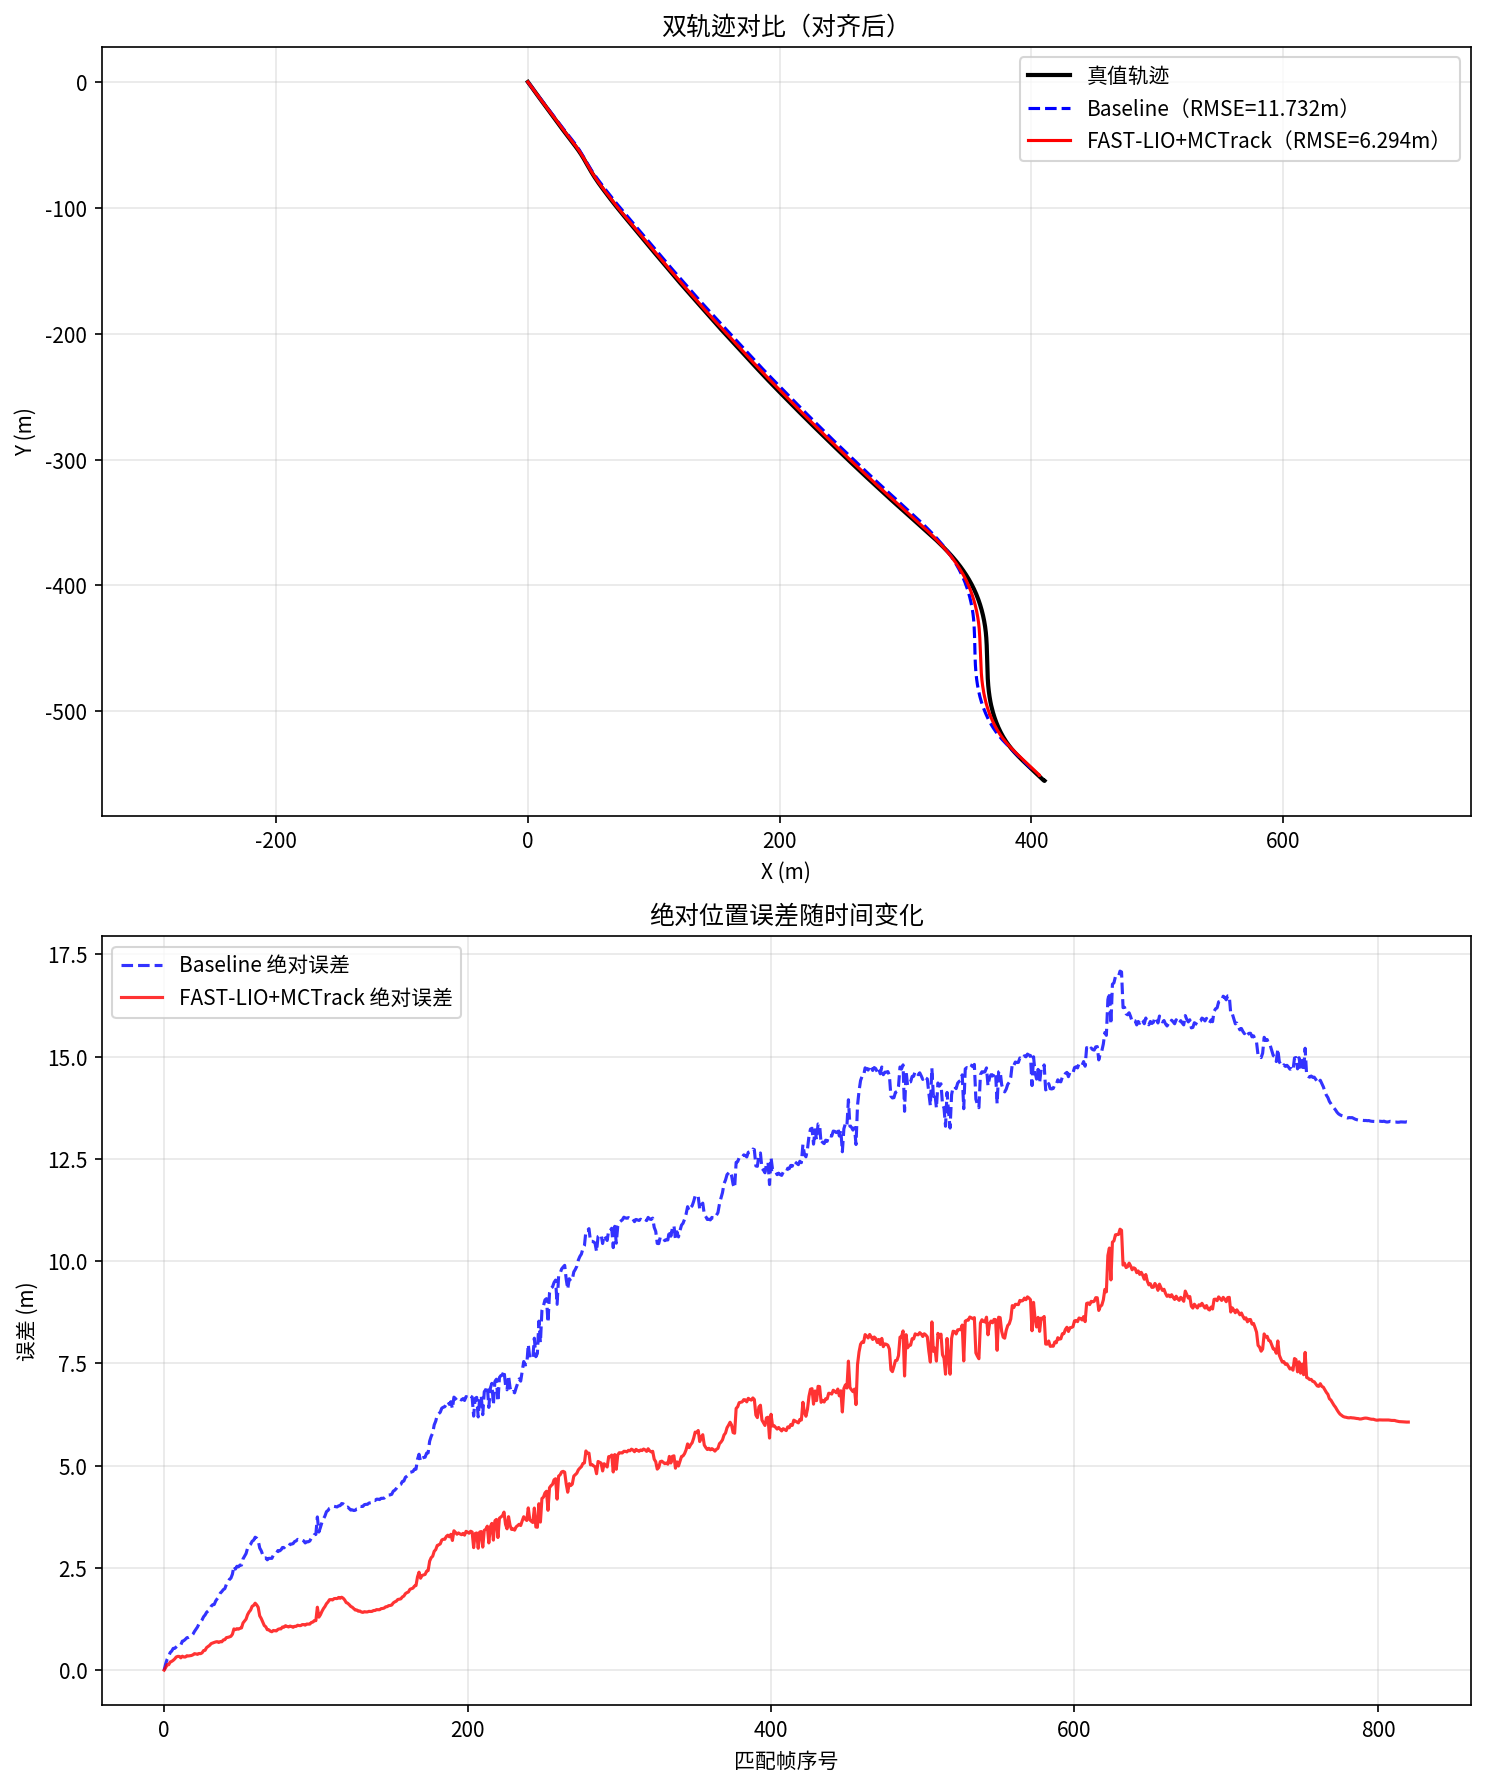
\includegraphics[width=0.72\textwidth]{../Results/0020_results/Online/evaluation_result.png}
    \caption{Online trajectory evaluation for Sequence 0020. The red \texttt{FAST-LIO+MCTrack} trajectory is clearly closer to the ground truth than the blue baseline.}
    \label{fig:online_0020_traj}
\end{figure}

\begin{figure}[H]
    \centering
    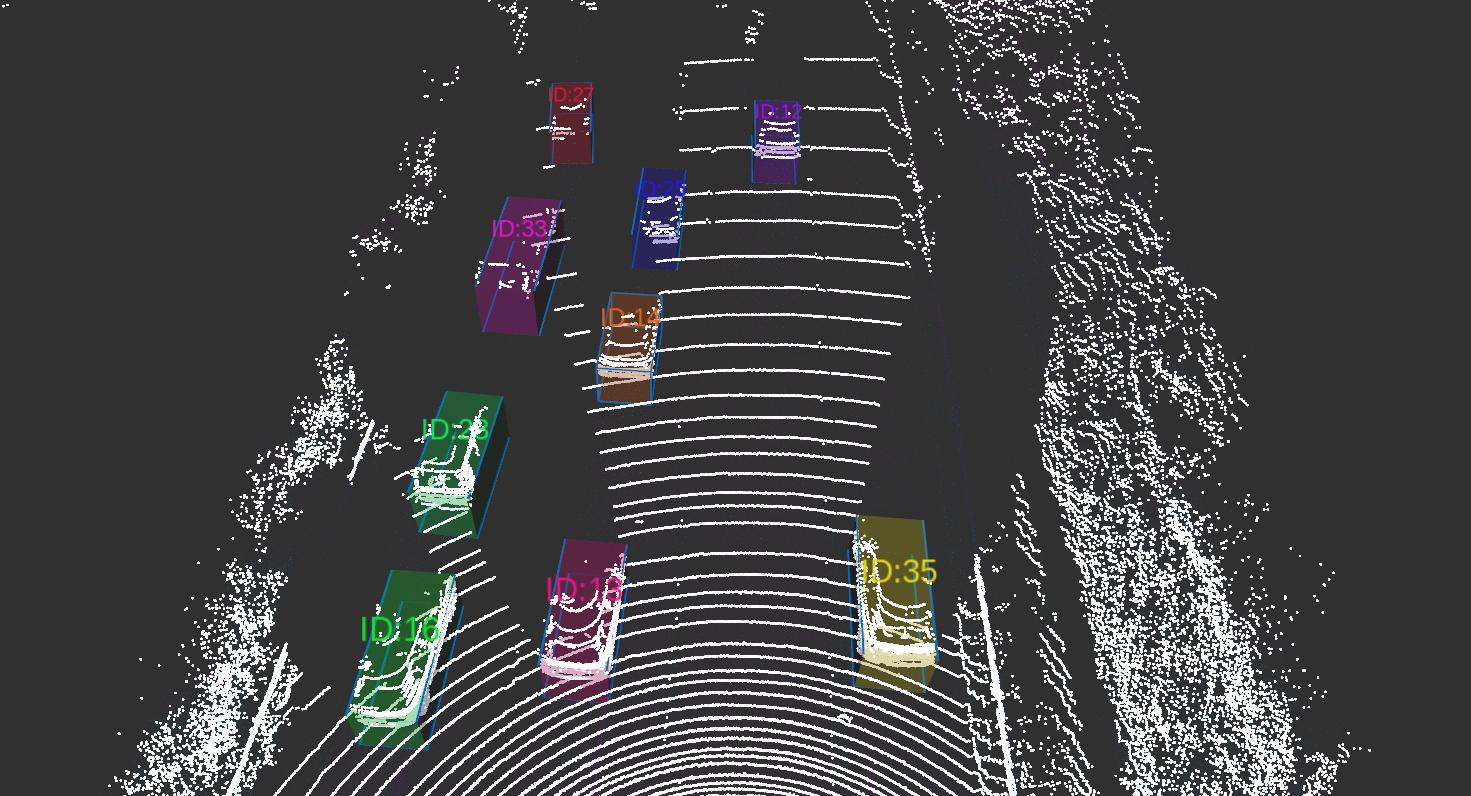
\includegraphics[width=0.72\textwidth]{Visualization of tracked dynamic vehicles on Sequence 0020.png}
    \caption{Dynamic-vehicle tracking visualization for Sequence 0020.}
    \label{fig:online_0020_tracking}
\end{figure}

\subsection{Integrated Analysis and Failure Modes}
\textbf{High dynamic scenes with large baseline drift: Sequences 0010 and 0020.} These two sequences are the clearest demonstrations of the current system's front-end value. In Sequence 0010, the baseline already suffers significant global deviation, and the front-end loop reduces ATE RMSE from 3.7651\,m to 0.8680\,m while also lowering RPE RMSE from 0.2774 to 0.2281. The joint backend remains good relative to baseline but is slightly worse than the front-end output, which suggests that most of the gain has already been captured before backend correction. Sequence 0020 shows a similar but longer-horizon pattern. The front-end loop cuts ATE RMSE from 11.7323\,m to 6.7938\,m and improves KITTI translation error from 3.2245\% to 2.3967\%. The backend preserves much of this global gain, but RPE changes only marginally. The most plausible explanation is that these sequences suffer from dynamic-scene contamination and global drift strongly enough that better front-end weighting yields a large benefit, while the backend has little clean additional information left to exploit.

\textbf{Moderate dynamic scenes: Sequences 0003 and 0006.} These two sequences show a subtler but extremely important pattern. The front-end loop improves both ATE and RPE: Sequence 0003 improves ATE RMSE by 14.75\%, and Sequence 0006 improves it by 10.09\%, with especially clear RPE improvement in 0006 from 0.1324 to 0.0869. Yet in both sequences the backend degrades performance, pushing ATE above baseline and noticeably worsening RPE and KITTI relative errors. This indicates that the front-end improvement is not merely a by-product of easier sequences. The front-end helps even in moderate cases. The backend failure in these sequences likely reflects over-correction: the baseline and front-end are already reasonably good, so a small number of noisy object factors can do more harm than good. In other words, the backend currently lacks a sufficiently strong activation criterion for deciding when object-derived correction is worth the risk.

\textbf{Low-dynamic or static-structure-rich scenes: Sequences 0007 and 0013.} These sequences are valuable because they test whether the proposed loop remains safe when the problem is not strongly dynamic. The answer is mostly yes for the front-end. Sequence 0007 shows a small ATE gain from 2.3128\,m to 2.2393\,m, and Sequence 0013 shows a modest but consistent ATE and RPE gain. The backend is nearly identical to the front-end in both cases, indicating that object-derived correction neither adds much nor causes serious damage. This is a useful outcome. It suggests that the front-end weighting loop does not require highly dramatic dynamic content in order to remain stable, while also showing that the backend has little positive leverage when the baseline is already comparatively well constrained by static structure.

\textbf{Backend failure case: Sequence 0009.} Sequence 0009 deserves to stand alone because its failure is qualitatively different from the moderate degradations seen elsewhere. The front-end loop makes a small but real improvement, reducing ATE RMSE from 1.6831\,m to 1.6675\,m and RPE RMSE from 0.1787 to 0.1651. The backend then collapses: ATE RMSE rises to 3.3082\,m, ATE max error reaches 40.3063\,m, KITTI translation error worsens from 2.5630\% to 4.2200\%, and RPE RMSE jumps to 1.9514. This pattern points to a localized but severe inconsistency being injected into the ego estimate. The likely root causes are exactly those discussed in the backend chapter: velocity extrapolation error, insufficiently strict gating, and timing mismatch between odometry and tracked objects. Sequence 0009 therefore functions as the anchor case proving that the backend is not merely ``less good than the front-end'' but can actively destabilize the trajectory if object evidence is trusted too much under the current design.

\subsection{From Observation to Explanation}
Taken together, the scene-grouped results support a reasonably clear mechanistic interpretation. When the baseline is mainly hurt by dynamic-object contamination in the front-end, the current system helps reliably because the front-end loop formed by pose-assisted tracking and tracking-feedback down-weighting likely interrupts that mechanism before registration and mapping errors accumulate. This is why the front-end loop improves all seven selected sequences and delivers the largest gains in drift-prone dynamic cases. It must be emphasized, however, that the present experiments do not fully disentangle the two internal mechanisms of that front-end loop. The more defensible conclusion is therefore that the front-end combination is effective as a whole, not that the gain has already been rigorously isolated and attributed primarily and uniquely to one individual module. When the baseline is already relatively stable, the backend has less room to help and more chance to inject noise through imperfect tracked-object constraints.

The difference between ATE and RPE trends is also instructive. On some sequences, the backend preserves a better global path shape while offering little or no RPE improvement, which is consistent with a low-frequency correction mechanism rather than a uniformly better local optimizer. The front-end remains stable because its use of object information is conservative and local, whereas the backend converts tracked-object information into stronger ego constraints and therefore demands much better synchronization, confidence modeling, and motion prediction quality.

\subsection{Experimental Fairness and Reporting Discipline}
Finally, the experimental conclusions are strengthened by the consistent comparison protocol across all reported sequences. The same archived data source, trajectory format, evaluation script, and result-directory convention are used for baseline, front-end, and backend comparisons. This matters when interpreting small gains versus large failures, because it reduces the chance that the trends come from post-processing differences rather than actual system behavior.

The main experimental conclusion is therefore clear at the level actually tested here. Within the seven selected online sequences and the current archived workflow, the project shows that front-end dynamic down-weighting driven by object-level information can improve SLAM localization error consistently across KITTI multi-sequence scenes. That object-aware front-end localization-enhancement path is the most reliable source of gain in the current system. The backend direction is promising but still immature, and its failures are informative rather than accidental. For a course project, this is a strong result: the system does not merely show that some improvement exists, but identifies where the improvement is robust, where it is fragile, and why the difference occurs.

\section{Conclusion and Future Plan}
This report reframes the ME5400 project as a technical study centered on one question: how to improve LiDAR SLAM localization accuracy in dynamic scenes while staying faithful to the actual repository state. The main achievement is not merely that FAST-LIO, PointPillars, and MCTrack have been assembled under one system label. Rather, the project builds a rerunnable object-aware localization-enhancement pipeline: FAST-LIO serves as the localization backbone, PointPillars and MCTrack provide object-level dynamic observations, front-end dynamic down-weighting applies those observations directly to scan matching, and the ego-only backend remains an exploratory extension for further reuse of object information. Combined with explicit ROS interfaces, scripted experiment orchestration, and archived evaluation on seven KITTI Tracking sequences, this yields an engineering validation platform for studying localization gains and failure mechanisms in dynamic driving scenes.

The most important verified conclusion is also the simplest. The most stable and reliable gain in the current system comes from the object-aware front-end localization path: FAST-LIO poses help MCTrack produce stable trajectories, and MCTrack outputs in turn provide soft suppression cues for FAST-LIO. This front-end configuration improves ATE RMSE on all seven reported online sequences and improves KITTI translation error on most of them. The most mature and best-supported technical conclusion should therefore remain at the level that object-aware front-end processing can stably improve localization accuracy in dynamic scenes, rather than claiming that the project has already achieved a full joint SLAMMOT optimizer. The observed behavior strongly suggests that tracking-feedback dynamic weighting is a key mechanism, because it improves scan matching and local-map consistency in a conservative, robust, online-compatible way; but without additional front-end ablation experiments, the more rigorous wording is to describe it as a key mechanism rather than the uniquely proven sole driver of the gain.

The report is equally clear about what has \emph{not} yet been solved. The current exploratory backend is not a robust object-centric optimizer. It is an ego-only sliding-window prototype that tests a valid idea under simplified assumptions. It can help on drift-dominated sequences, but it can also degrade badly when object velocity extrapolation, time alignment, or gating are imperfect. Sequence 0009 is the key reminder that reusing tracked objects as positive localization constraints is substantially harder than merely using them for soft front-end suppression. This is not a contradiction of the project hypothesis. It is the exact evidence needed to refine that hypothesis into a stronger next-stage design.

The future work can therefore be prioritized rather clearly. \textbf{First}, the backend should evolve from an ego-only corrector into an \textbf{object-centric joint backend} in which object states are optimized together with ego pose instead of entering only as external observations. This is the most important upgrade because it directly addresses the current inability to absorb object-state error inside the optimization. \textbf{Second}, the system needs \textbf{stronger confidence modeling and association strategy}. Detection score and track length are useful first heuristics, but they are not sufficient for deciding when an object factor should influence ego motion strongly. Confidence-aware weighting, more explicit motion consistency checks, and richer data-association diagnostics are all needed. \textbf{Third}, the system needs \textbf{richer motion modeling for tracked objects}. If object states are to move from front-end support into stable backend constraints, one constant-velocity extrapolation is clearly not enough; vehicle turning, stop-and-go behavior, and participant-dependent dynamics all need better representation. \textbf{Fourth}, the project should be validated on \textbf{more KITTI Tracking sequences and traffic scenes with richer dynamic intensity} so that the current ``stable front end, fragile backend'' pattern can be tested for broader scene stability.

From the perspective of course value, this is a strong and honest outcome. The project has already integrated multiple complex modules into one coherent workflow, shown that object-level dynamic information can produce stable front-end localization gains, and exposed the real engineering gaps that block a stronger joint backend. That combination of working system, rerunnable experiments within the current repository workflow, and transparent failure analysis is precisely what makes the current prototype useful for continued research. If the next iteration succeeds in promoting today's message-level object feedback into a true object-centric localization graph, the project can evolve naturally from a course-scale engineering validation into a more substantive research contribution on dynamic-scene LiDAR SLAM localization enhancement.

\clearpage
\addcontentsline{toc}{section}{References}
\begin{thebibliography}{99}
\bibitem{fastlio2}
W. Xu, Y. Cai, D. He, J. Lin, and F. Zhang, ``FAST-LIO2: Fast direct LiDAR-inertial odometry,'' \emph{IEEE Transactions on Robotics}, vol. 38, no. 4, pp. 2053--2073, 2022.

\bibitem{pointpillars}
A. H. Lang, S. Vora, H. Caesar, L. Zhou, J. Yang, and O. Beijbom, ``PointPillars: Fast encoders for object detection from point clouds,'' in \emph{Proc. CVPR}, 2019, pp. 12697--12705.

\bibitem{mctrack}
X. Wang, S. Qi, J. Zhao, H. Zhou, S. Zhang, G. Wang, K. Tu, S. Guo, J. Zhao, J. Li, and M. Yang, ``MCTrack: A Unified 3D Multi-Object Tracking Framework for Autonomous Driving,'' in \emph{Proc. IROS}, 2025.

\bibitem{kitti}
A. Geiger, P. Lenz, and R. Urtasun, ``Are we ready for autonomous driving? The KITTI vision benchmark suite,'' in \emph{Proc. CVPR}, 2012, pp. 3354--3361.

\bibitem{staticfusion}
R. Scona, M. Jaimez, Y. R. Petillot, M. Fallon, and D. Cremers, ``StaticFusion: Background reconstruction for dense RGB-D SLAM in dynamic environments,'' in \emph{Proc. ICRA}, 2018.

\bibitem{ds-slam}
C. Yu, Z. Liu, X. Liu, F. Xie, Y. Yang, Q. Wei, and Q. Fei, ``DS-SLAM: A semantic visual SLAM towards dynamic environments,'' in \emph{Proc. IROS}, 2018.

\bibitem{dynaslam}
B. Bescos, J. M. Facil, J. Civera, and J. Neira, ``DynaSLAM: Tracking, mapping and inpainting in dynamic scenes,'' \emph{IEEE Robotics and Automation Letters}, vol. 3, no. 4, 2018.

\bibitem{confslammot}
S. Fang and H. Li, ``LiDAR SLAMMOT based on Confidence-guided Data Association,'' \emph{arXiv preprint arXiv:2412.01041}, 2024.

\bibitem{limot}
Z. Zhu, J. Zhao, K. Huang, X. Tian, J. Lin, and C. Ye, ``LIMOT: A Tightly-Coupled System for LiDAR-Inertial Odometry and Multi-Object Tracking,'' \emph{IEEE Robotics and Automation Letters}, vol. 9, no. 7, pp. 6600--6607, 2024.

\bibitem{imm-slammot}
P. Tian and H. Li, ``Visual SLAMMOT Considering Multiple Motion Models,'' \emph{arXiv preprint arXiv:2411.19134}, 2024.

\bibitem{online-dynamic-slam}
J. Morris, Y. Wang, and V. Ila, ``Online Dynamic SLAM with Incremental Smoothing and Mapping,'' \emph{arXiv preprint arXiv:2509.08197}, 2025.

\bibitem{dl-slot}
X. Tian, Z. Zhu, J. Zhao, G. Tian, and C. Ye, ``DL-SLOT: Tightly-Coupled Dynamic LiDAR SLAM and 3D Object Tracking Based on Collaborative Graph Optimization,'' \emph{IEEE Transactions on Intelligent Vehicles}, vol. 9, no. 1, pp. 1017--1027, 2024.

\bibitem{ab3dmot}
X. Weng, J. Wang, D. Held, and K. Kitani, ``3D multi-object tracking: A baseline and new evaluation metrics,'' in \emph{Proc. IROS}, 2020, pp. 10359--10366.

\bibitem{centerpoint}
T. Yin, X. Zhou, and P. Krahenbuhl, ``Center-based 3D object detection and tracking,'' in \emph{Proc. CVPR}, 2021, pp. 11784--11793.

\end{thebibliography}

\clearpage
\section*{Acknowledgment}
\addcontentsline{toc}{section}{Acknowledgment}
As I complete this report for the ME5400 project, I would like to express my sincere gratitude to everyone who has supported me throughout this work. This report is not only a summary of the project itself, but also a meaningful record of my learning, research, and engineering practice during my study.

First of all, I would like to thank all the teachers in the College of Design and Engineering at the National University of Singapore for their teaching, guidance, and academic support during my master's study. Their patience and dedication have greatly deepened my understanding of both research and engineering practice.

I am especially grateful to my supervisor, Professor Marcelo H. Ang Jr., for his valuable guidance and support throughout this project. I would also like to sincerely thank Professor Teo Chee Leong for his time and thoughtful evaluation of this work. My heartfelt thanks also go to Han Yuhang, whose guidance was of great help during this research, and to every member of our research group for their companionship, discussions, and encouragement.

Finally, I would like to express my deepest respect and gratitude to my family and friends. Their love, trust, and support have always given me strength, especially during difficult and uncertain moments.

As I move forward into future work and life beyond school, I will carry this kindness with me and continue my journey with sincerity, gratitude, and hope.

\clearpage
\appendix
\section*{Appendix: All Online Experimental Figures}
\addcontentsline{toc}{section}{Appendix: All Online Experimental Figures}
This appendix inserts all online result figures by sequence. Each sequence includes the online front-end comparison, the joint-backend evaluation, and the bar-chart comparison.

\onlineResultFigure{0003}
\onlineResultFigure{0006}
\onlineResultFigure{0007}
\onlineResultFigure{0009}
\onlineResultFigure{0010}
\onlineResultFigure{0013}
\onlineResultFigure{0020}

\end{document}
